\documentclass[12pt]{article}
\usepackage[margin=1in]{geometry}
\usepackage{setspace}
\doublespacing
\usepackage{graphicx}
\usepackage{booktabs}
\usepackage{amsmath}
\usepackage{amssymb}
\usepackage{caption}
\usepackage{float}
\usepackage{hyperref}
\usepackage{natbib}

\newcommand{\sym}[1]{\textsuperscript{#1}}

\hypersetup{
    colorlinks=true,
    linkcolor=black,
    citecolor=black,
    urlcolor=blue
}

\title{Local Income Taxes and Residential Sorting: \\
\large Evidence from LEHD Origin-Destination Data}
\author{Matthew Hockert\thanks{University of Minnesota. Email: hocke043@umn.edu}}
\date{\today}

\begin{document}

\maketitle

\begin{abstract}
% TODO: Write abstract
\end{abstract}

\newpage

%==========================================================
\section{Introduction}
\label{sec:intro}
%==========================================================
% TODO: Tiebout hypothesis, gap in within-metro sorting evidence,
% LODES OD contribution, fiscal incidence punchline.
% Key framing: "employment becomes less locally resident"
% Three contributions: (1) new measure, (2) causal evidence, (3) fiscal incidence
%
% Suggested reviewer framing:
% "Local income tax increases reduce the locally resident share of city workers,
%  implying modest residential sorting away from taxed municipalities. But the
%  behavioral response is too small to offset the fiscal gains from higher rates."

%==========================================================
\section{Institutional Background}
\label{sec:background}
%==========================================================

\subsection{Ohio Municipal Income Tax}
\label{subsec:ohio}
% TODO: 685 municipalities with rates 0--3%, unincorporated townships have no tax.
% 302 rate increases, 45 decreases in our panel (2002--2019).

\subsection{Pennsylvania Earned Income Tax}
\label{subsec:pennsylvania}
% TODO: Mandatory EIT for all 2,500+ municipalities under Local Tax Enabling Act.
% Standard cap: 1% split (typically 0.5% muni / 0.5% school district).
% Home Rule municipalities can exceed (Philadelphia at ~4.3%).
% Property tax millage cap forces EIT as primary revenue lever.
% EIT and property tax changes uncorrelated (r = -0.04).
% EIT applies to all earned income, no minimum threshold. Retirees exempt.
% 291 rate increases, 162 decreases in panel.

%==========================================================
\section{Data}
\label{sec:data}
%==========================================================

\subsection{LODES Origin-Destination Data}
\label{subsec:lodes}
% TODO: LEHD LODES8, 2002--2019 (trim 2020--2021 due to COVID).
% Tract-level residence-workplace links. Aggregated to municipality level.
% Cross-state aux flows included. Segments: S000, SE01, SE03, SA01--SA03.
% Reference date: April 1. Noise infusion at block level, aggregation reduces.

\subsection{Municipal Tax Rate Panels}
\label{subsec:rates}
% TODO: OH from Dept of Taxation ``The Finder'' CSV. Direct PLACEFP join.
% PA from DCED MunStats scraped XLS (2000--2026). Name-based crosswalk to COUSUBFP (97\% match).
% April 1 alignment: rate active on April 1 of year Y = LODES year Y.

\subsection{Municipal Financial Reports}
\label{subsec:afr}
% TODO: PA DCED Annual Financial Reports, 2002--2019. 71 columns.
% EIT revenue, RE tax, police, streets, debt, state aid, population, market value RE.

\subsection{Outcome Variable: share\_live\_in}
\label{subsec:outcome}
% TODO: share_live_in = live_and_work / total_jobs.
% Fraction of workers employed in municipality who also reside there.
% Captures within-county, cross-municipal sorting invisible to IRS SOI/ACS.

% --- Summary Statistics Table ---
\begin{table}[H]
    \centering
    \caption{Summary Statistics}
    \label{tab:summary}
    \small
    \begin{tabular}{lrrrrr}
        \toprule
        Variable & Mean & Median & SD & Min & Max \\
        \midrule
        \multicolumn{6}{l}{\textit{Panel A: Pennsylvania (2002--2019)}} \\
        share\_live\_in              & 0.149  & 0.127  & 0.097 & 0     & 0.700 \\
        Resident EIT rate (\%)      & 0.542  & 0.500  & 0.199 & 0     & 4.331 \\
        Total jobs                  & 3{,}624 & 1{,}224 &       &       &       \\
        Resident workers            & 674    & 154    &       &       &       \\
        \midrule
        \multicolumn{6}{l}{\textit{Panel B: Ohio (2002--2019)}} \\
        share\_live\_in              & 0.119  & 0.099  & 0.085 &       &       \\
        Municipal tax rate (\%)     & 1.222  & 1.500  & 0.821 & 0     & 3.000 \\
        \midrule
        \multicolumn{6}{l}{\textit{Panel dimensions}} \\
        PA municipality $\times$ years & \multicolumn{5}{l}{24{,}528 (1{,}383 municipalities)} \\
        OH municipality $\times$ years & \multicolumn{5}{l}{7{,}718 (430 municipalities)} \\
        \bottomrule
    \end{tabular}
    \vspace{0.3em}
    \begin{minipage}{0.85\textwidth}
        \footnotesize \textit{Notes:} Municipality-year panel, 2002--2019.
        Sample restricted to municipalities with $>50$ total jobs.
        share\_live\_in = workers who live and work in municipality / total workers in municipality.
        OH municipalities are Census places; PA municipalities are county subdivisions.
    \end{minipage}
\end{table}

% --- Treatment Geography Figures ---
\begin{figure}[H]
    \centering
    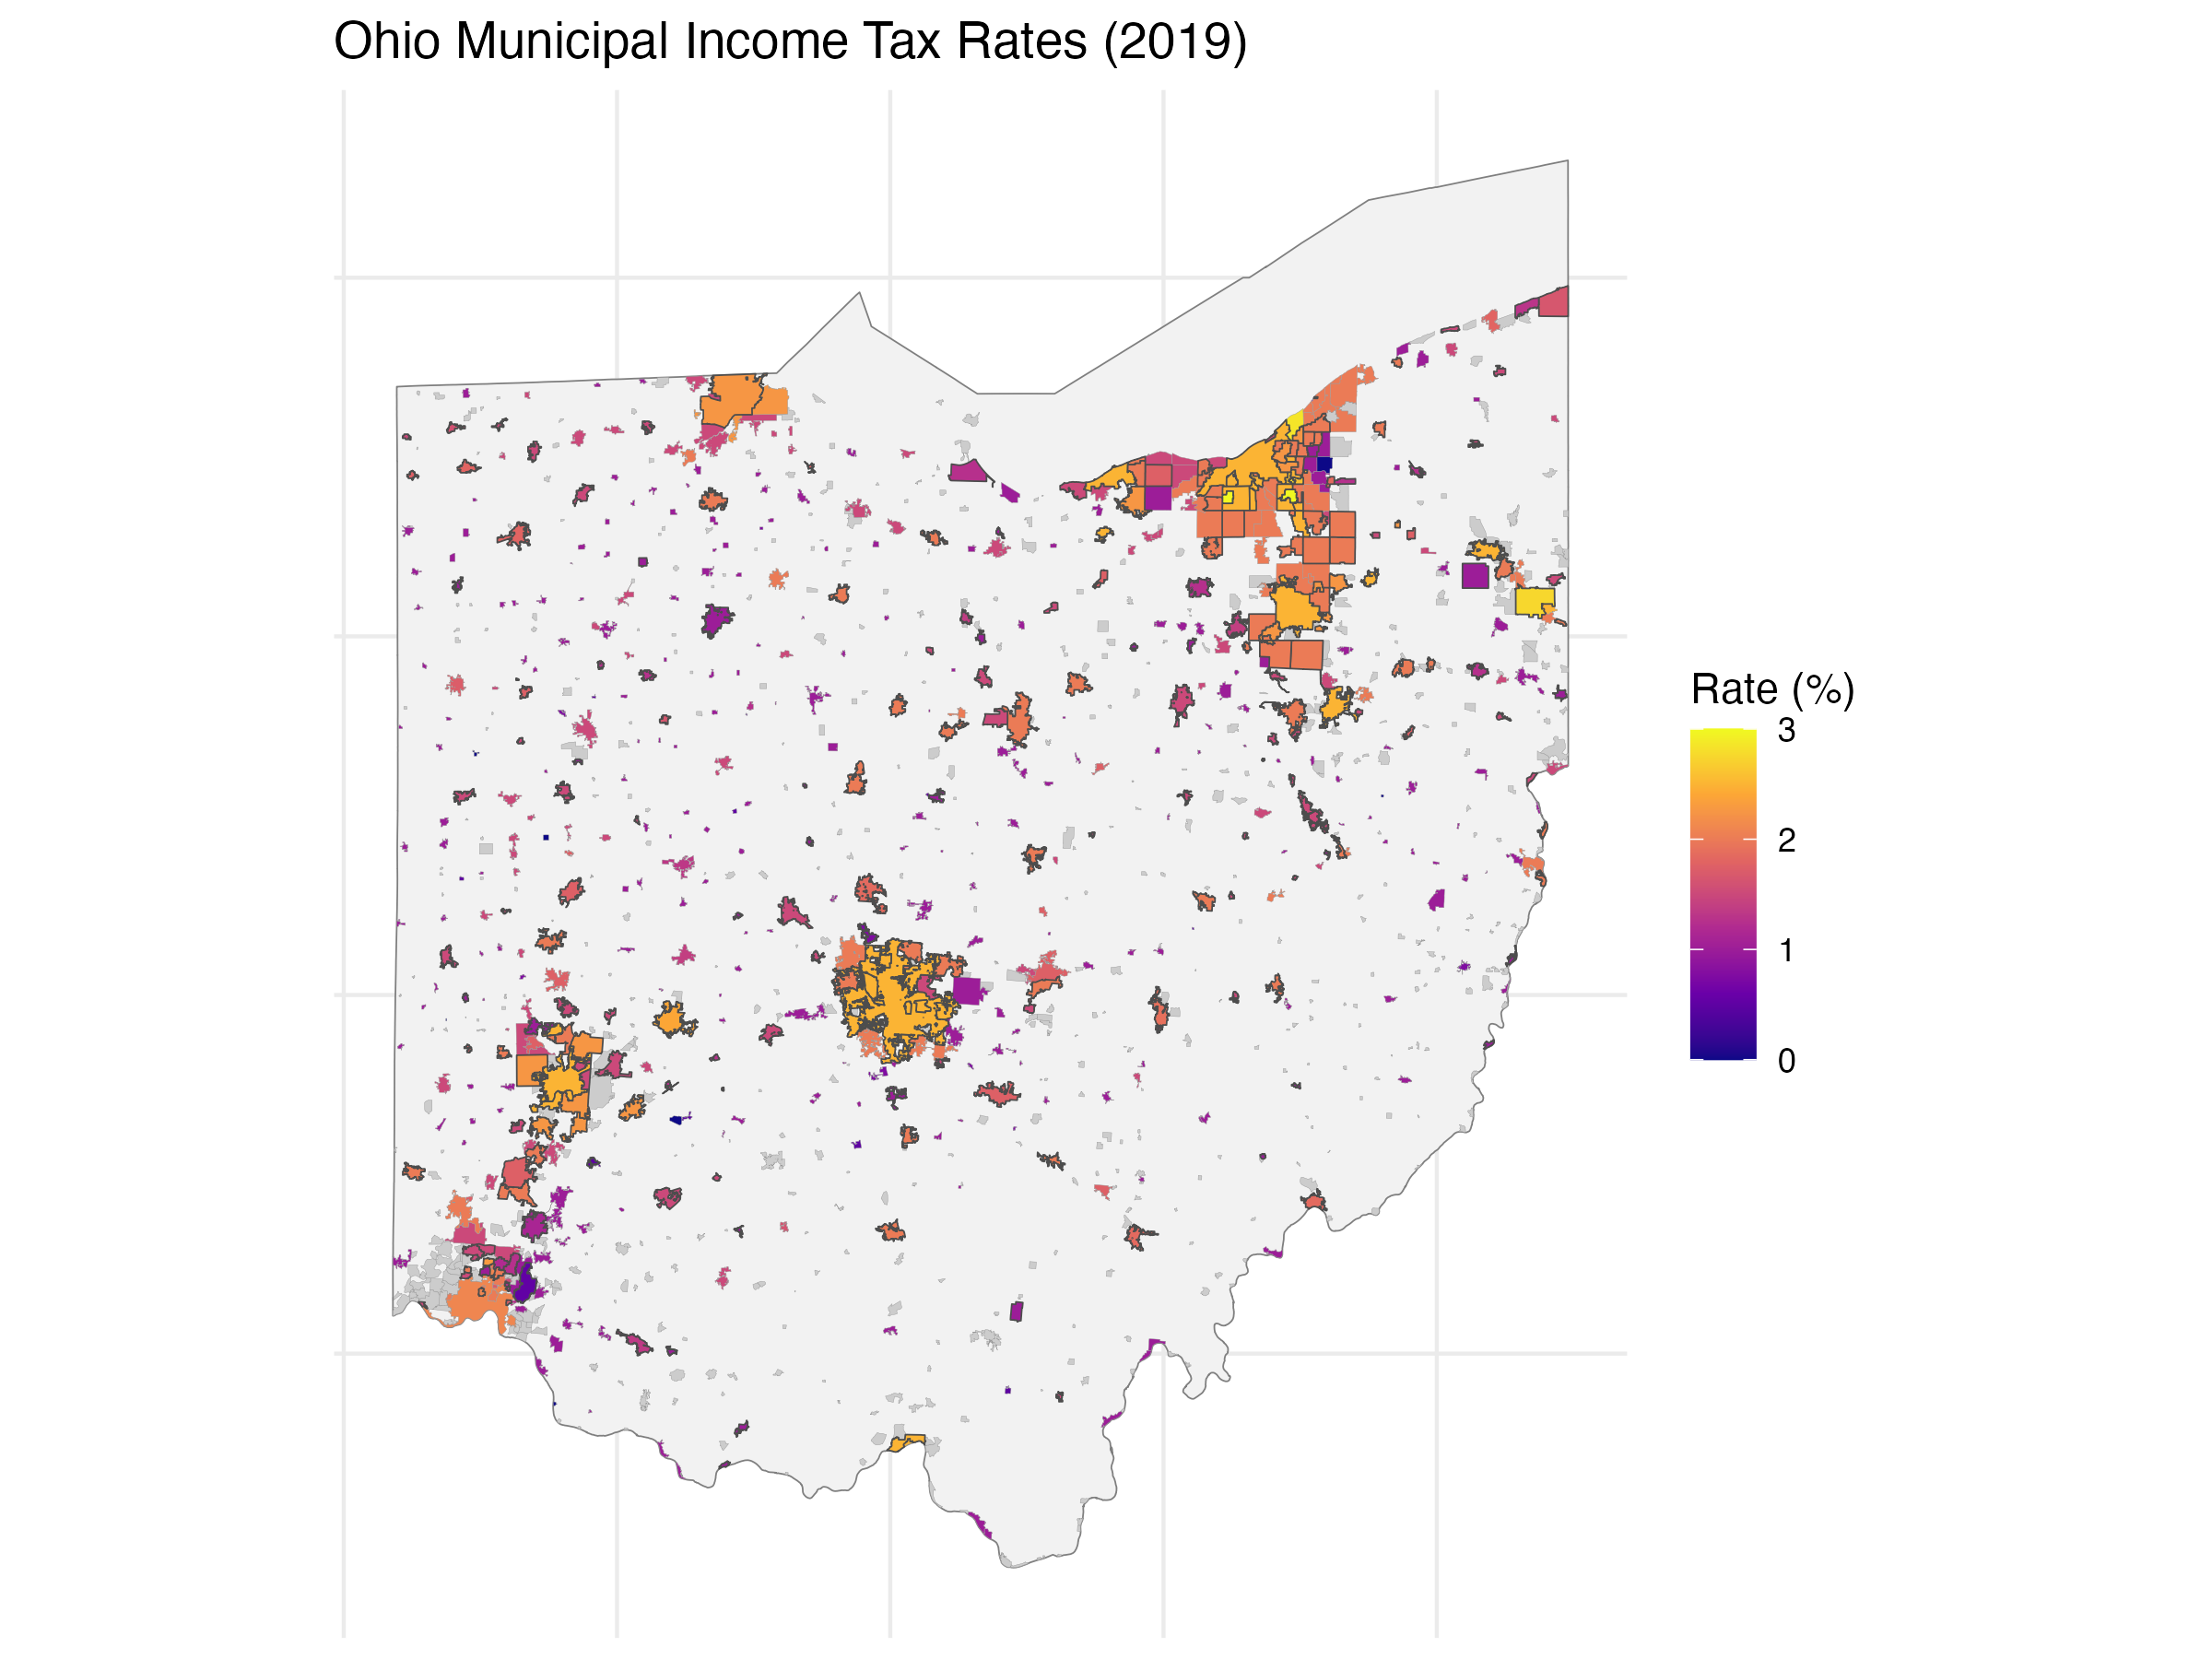
\includegraphics[width=0.85\textwidth]{../figures/oh_map.png}
    \caption{Ohio Municipal Income Tax Rates (2019). Bold outline = municipalities that raised rates during the sample period. Grey fill = municipalities with no municipal income tax.}
    \label{fig:oh_map}
\end{figure}

\begin{figure}[H]
    \centering
    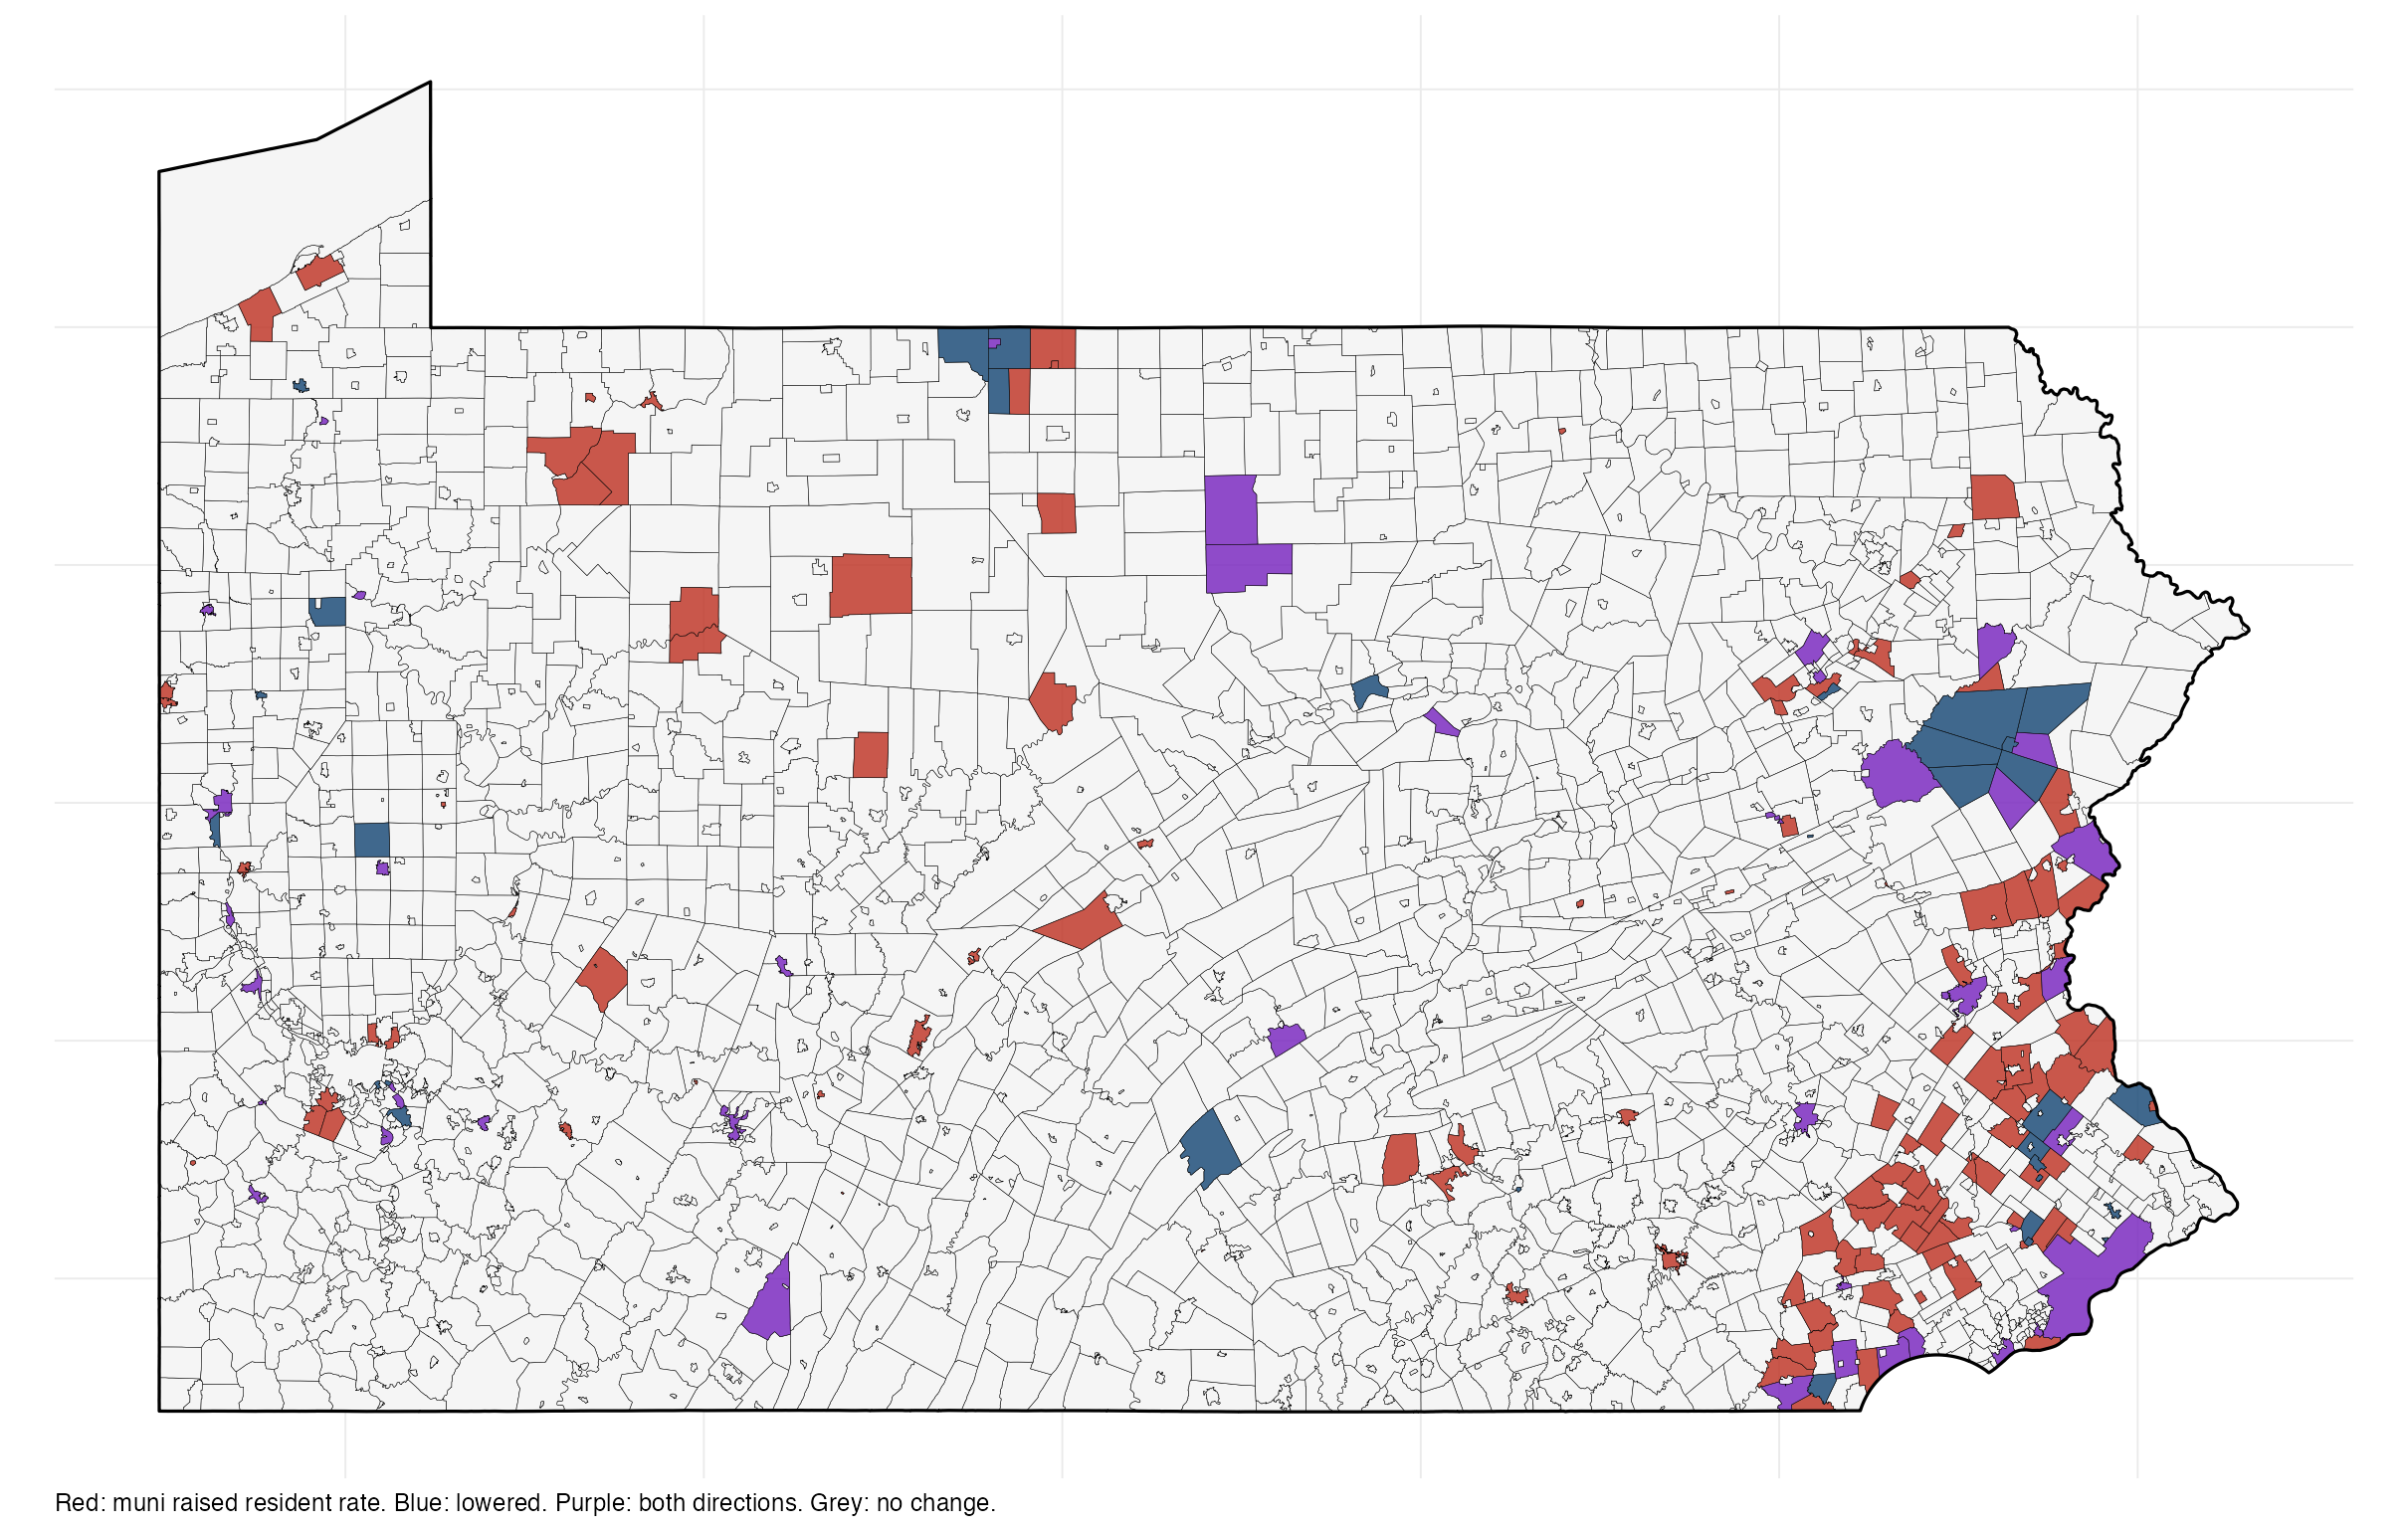
\includegraphics[width=0.85\textwidth]{../figures/pa_map.png}
    \caption{Pennsylvania EIT Rate Changes (2000--2019). Red = increased; blue = decreased; purple = both; grey = no change.}
    \label{fig:pa_map}
\end{figure}

\begin{figure}[H]
    \centering
    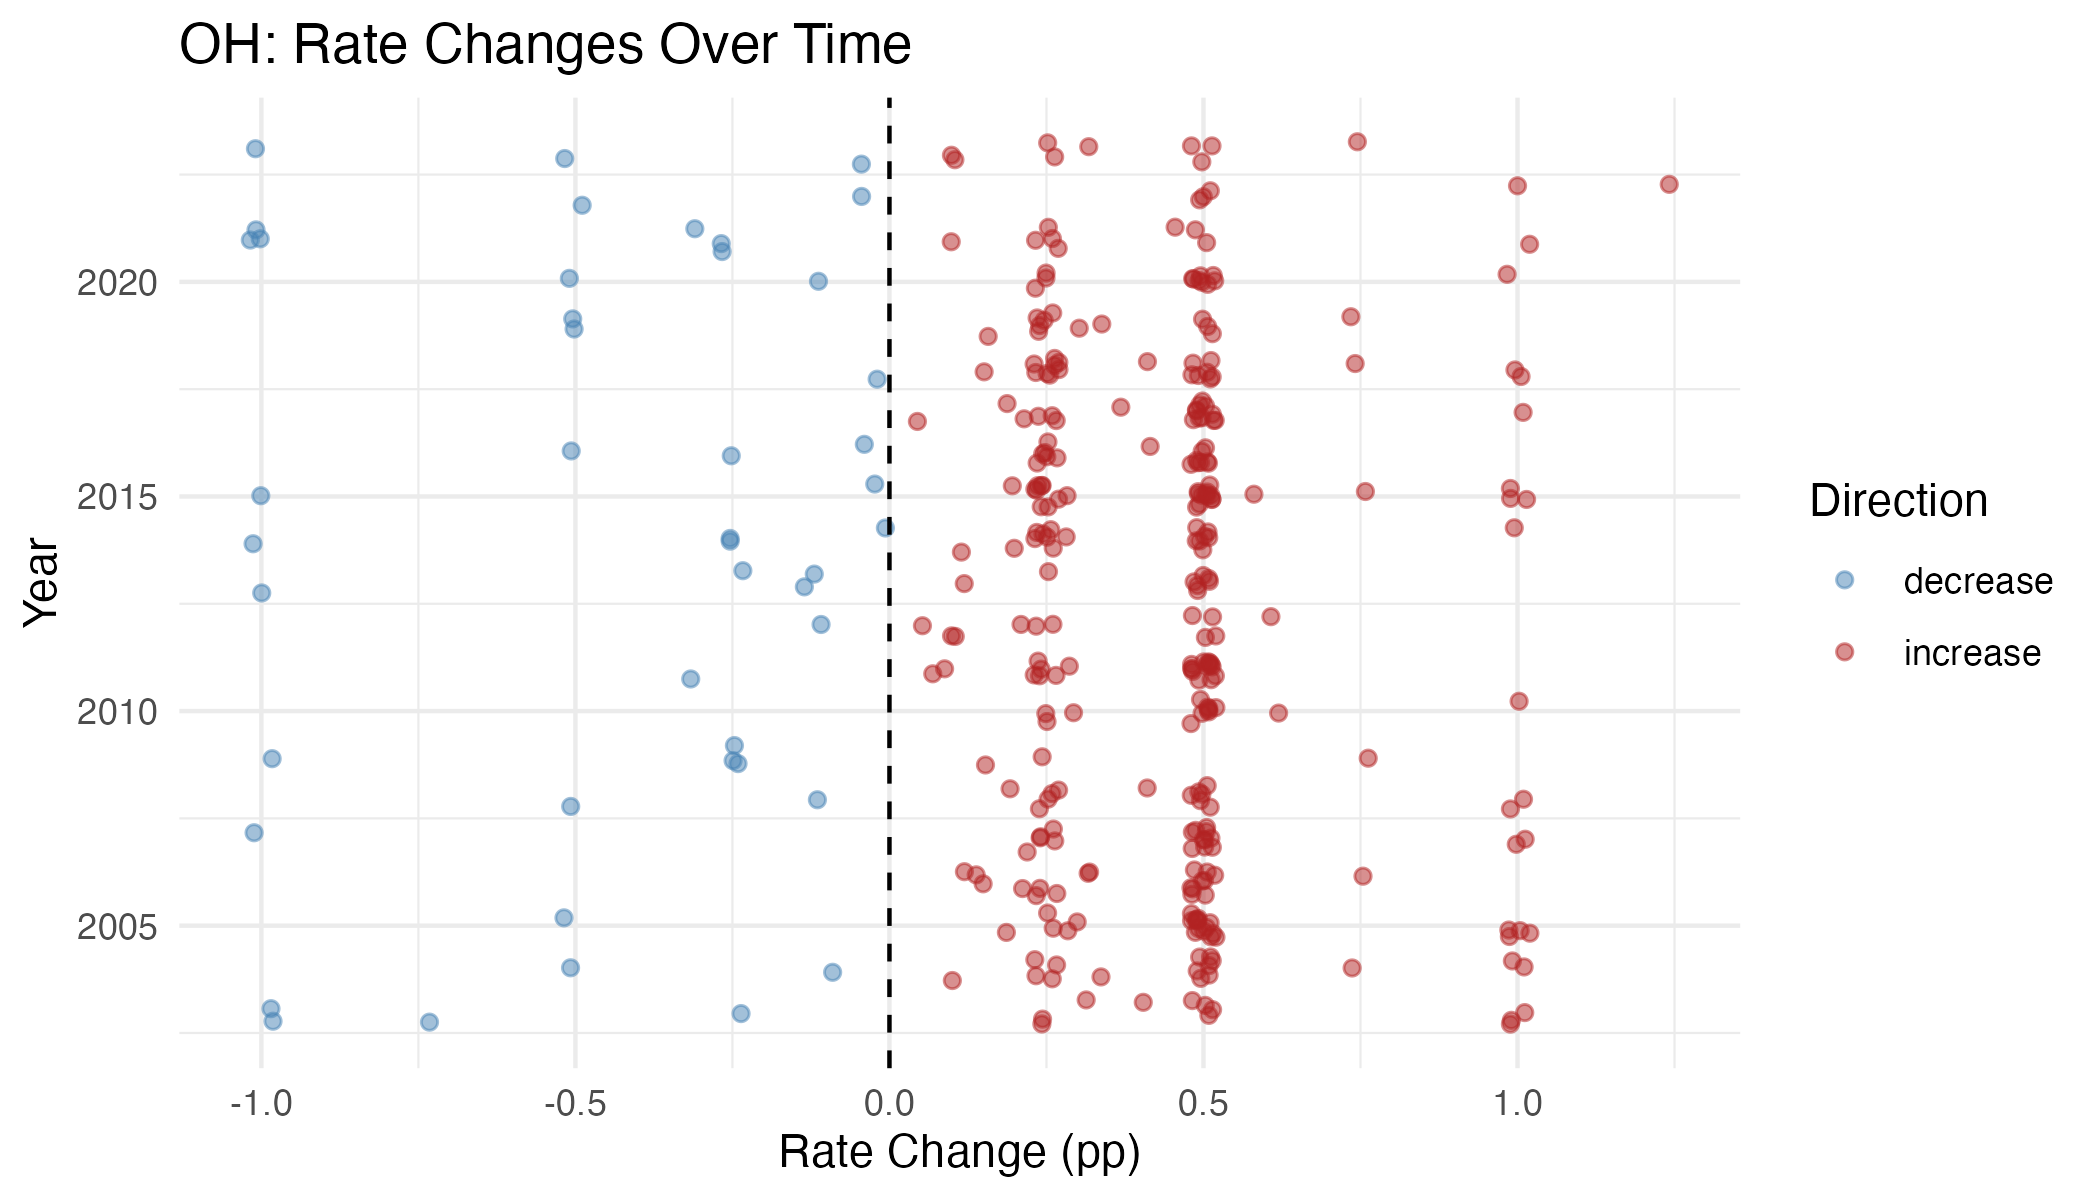
\includegraphics[width=0.75\textwidth]{../figures/oh_rate_scatter.png}
    \caption{Ohio: Distribution of Municipal Income Tax Rate Changes Over Time}
    \label{fig:oh_rate_scatter}
\end{figure}

\begin{figure}[H]
    \centering
    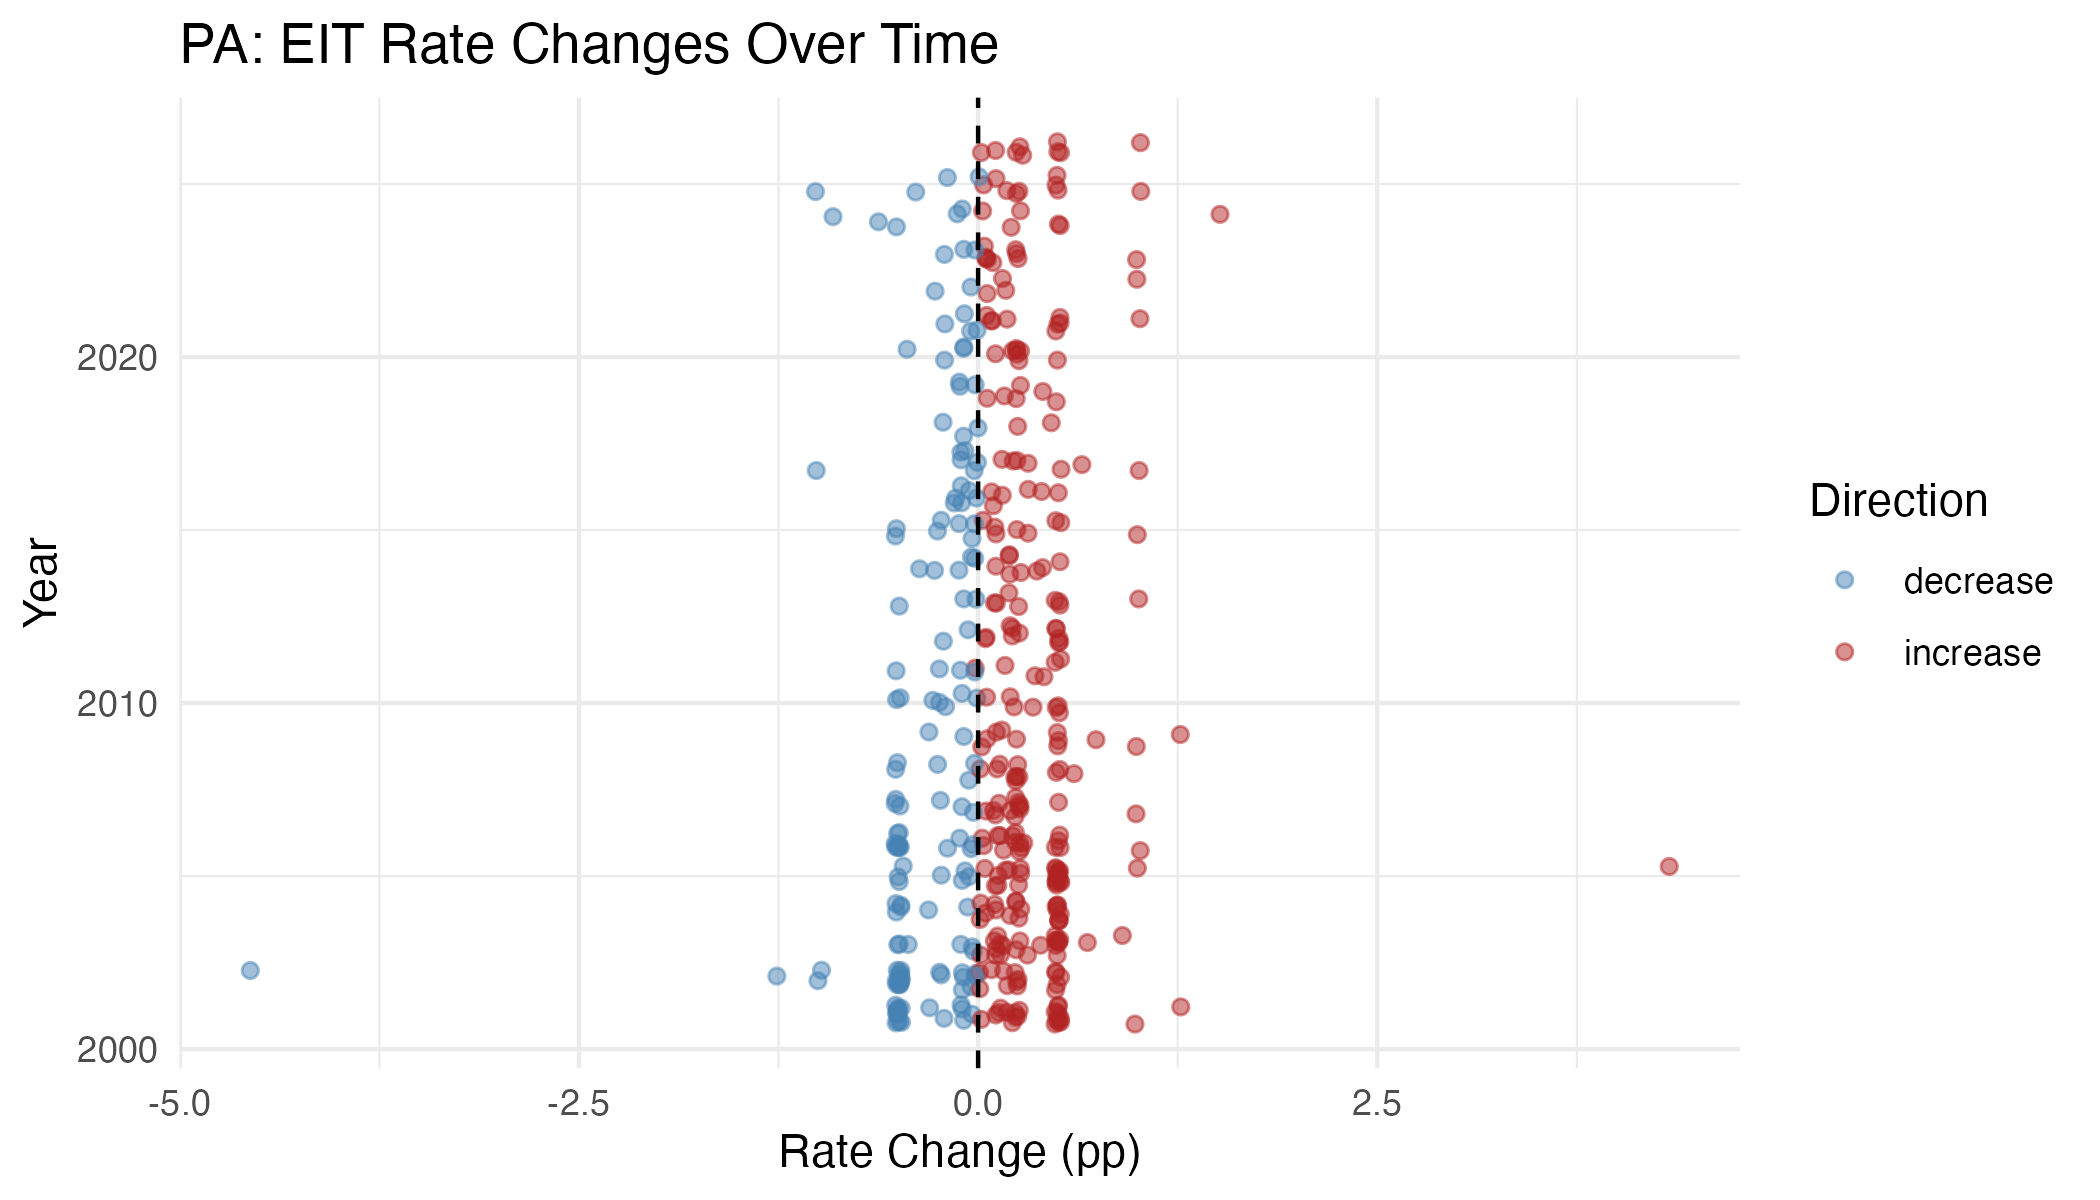
\includegraphics[width=0.75\textwidth]{../figures/pa_rate_scatter.png}
    \caption{Pennsylvania: Distribution of EIT Rate Changes Over Time}
    \label{fig:pa_rate_scatter}
\end{figure}

%==========================================================
\section{Empirical Strategy}
\label{sec:strategy}
%==========================================================

We organize our analysis around four questions, each building on the
previous. All specifications use municipality and year fixed effects
with standard errors clustered at the municipality level. For binary
treatments under staggered timing, we use the Sun and Abraham (2021)
interaction-weighted estimator:

\begin{equation}
    Y_{it} = \alpha_i + \gamma_t + \sum_{\ell \neq -1} \mu_\ell \cdot D_{it}^{\ell} + \mathbf{X}'_{it}\boldsymbol{\phi} + \varepsilon_{it}
    \label{eq:sunab}
\end{equation}

\noindent where $Y_{it}$ is share\_live\_in, $D_{it}^{\ell}$ indicates
municipality $i$ being $\ell$ years from its first treatment, and
$\mathbf{X}_{it}$ is a vector of fiscal controls (available for PA).
Pre-treatment coefficients ($\ell < -1$) test parallel trends. For
continuous treatments (the actual tax rate), we use the de Chaisemartin
and D'Haultfoeuille (2024) estimator, which handles both staggered
timing and varying treatment intensity.

\paragraph{Q1: Does adopting a local income tax cause residential sorting?}
Ohio municipalities can adopt a local income tax; unincorporated
townships have no tax. We compare municipalities that adopted a tax
during the panel (going from 0 to a positive rate) against no-tax
townships. This is the cleanest Tiebout test: a discrete switch from
no tax to having one. Only Ohio provides this extensive-margin variation;
all Pennsylvania municipalities levy an EIT throughout the panel.

\paragraph{Q2: Do rate increases cause additional sorting?}
Conditional on already having a tax, does raising the rate push
additional residents out? We estimate Equation~\ref{eq:sunab} with
rate increasers as the treated group. For Ohio, we use no-tax townships
as the control group (stable-rate taxed cities produce null results,
likely because they share unobserved urban characteristics with treated
cities). For Pennsylvania, the control group is the 2,209 municipalities
that never changed their EIT rate. We also estimate the DCDH continuous
treatment model, which tests whether rate \textit{magnitude} predicts
sorting beyond the binary treatment effect.

\paragraph{Q3: Do rate decreases reverse sorting?}
We estimate Equation~\ref{eq:sunab} with rate decreasers as the treated
group and never-changed municipalities as controls. If sorting is
reversible, decreases should increase the locally-resident share.

\paragraph{Q4: Is the sorting response asymmetric?}
We test whether increases and decreases have symmetric effects using
a joint model with both indicators and a split cumulative dose
specification:

\begin{equation}
    Y_{it} = \alpha_i + \gamma_t
    + \beta^{+} \cdot R^{+}_{it}
    + \beta^{-} \cdot R^{-}_{it}
    + \mathbf{X}'_{it}\boldsymbol{\phi} + \varepsilon_{it}
    \label{eq:split_dose}
\end{equation}

\noindent where $R^{+}_{it}$ and $R^{-}_{it}$ are cumulative rate
increases and decreases from baseline. If $|\beta^{+}| > |\beta^{-}|$,
residential location decisions are sticky: tax increases push residents
out, but tax decreases do not pull them back.


%==========================================================
\section{Results}
\label{sec:results}
%==========================================================

\subsection{Q1: Does Adopting a Tax Cause Sorting?}
\label{subsec:q1}

We pool municipalities from both states that adopted a local income tax
during the panel (going from a zero rate to a positive rate) and compare
them to municipalities that never levied a tax. Only 8 municipalities
adopted a tax and appear in the LODES data with sufficient employment:
1 in Ohio and 7 in Pennsylvania. The control group consists of 109
never-taxed municipalities (104 Ohio townships, 5 Pennsylvania
municipalities). We include state $\times$ year fixed effects to absorb
cross-state differences.

\begin{table}[H]
    \centering
    \caption{Q1: Effect of Tax Adoption on share\_live\_in}
    \label{tab:q1}
    \small
    \begin{tabular}{lc}
        \toprule
        & Pooled (OH + PA) \\
        \midrule
        Sun-Abraham ATT        & $-0.0036$    \\
                               & (0.0066)     \\
        \midrule
        Treated                & 8 adopters (1 OH, 7 PA) \\
        Control                & 109 never-taxed (104 OH, 5 PA) \\
        Fixed Effects          & Municipality, State $\times$ Year \\
        Clusters               & Municipality \\
        Min.\ total jobs       & 10 \\
        \bottomrule
    \end{tabular}
    \vspace{0.3em}
    \begin{minipage}{0.80\textwidth}
        \footnotesize \textit{Notes:} Sun-Abraham ATT from pooled OH and
        PA sample. Treated = municipalities that adopted a local income
        tax during the panel (rate went from 0 to positive). Control =
        municipalities that never levied a tax in either state. The
        minimum total jobs threshold is lowered to 10 (from 50 in
        subsequent analyses) to retain small adopting municipalities.
        Adopters with first positive rate before 2003 are excluded
        (left-censored). The small treatment group (8 municipalities)
        limits statistical power.
        \sym{.}$p<0.10$, \sym{*}$p<0.05$, \sym{**}$p<0.01$, \sym{***}$p<0.001$.
    \end{minipage}
\end{table}

\begin{figure}[H]
    \centering
    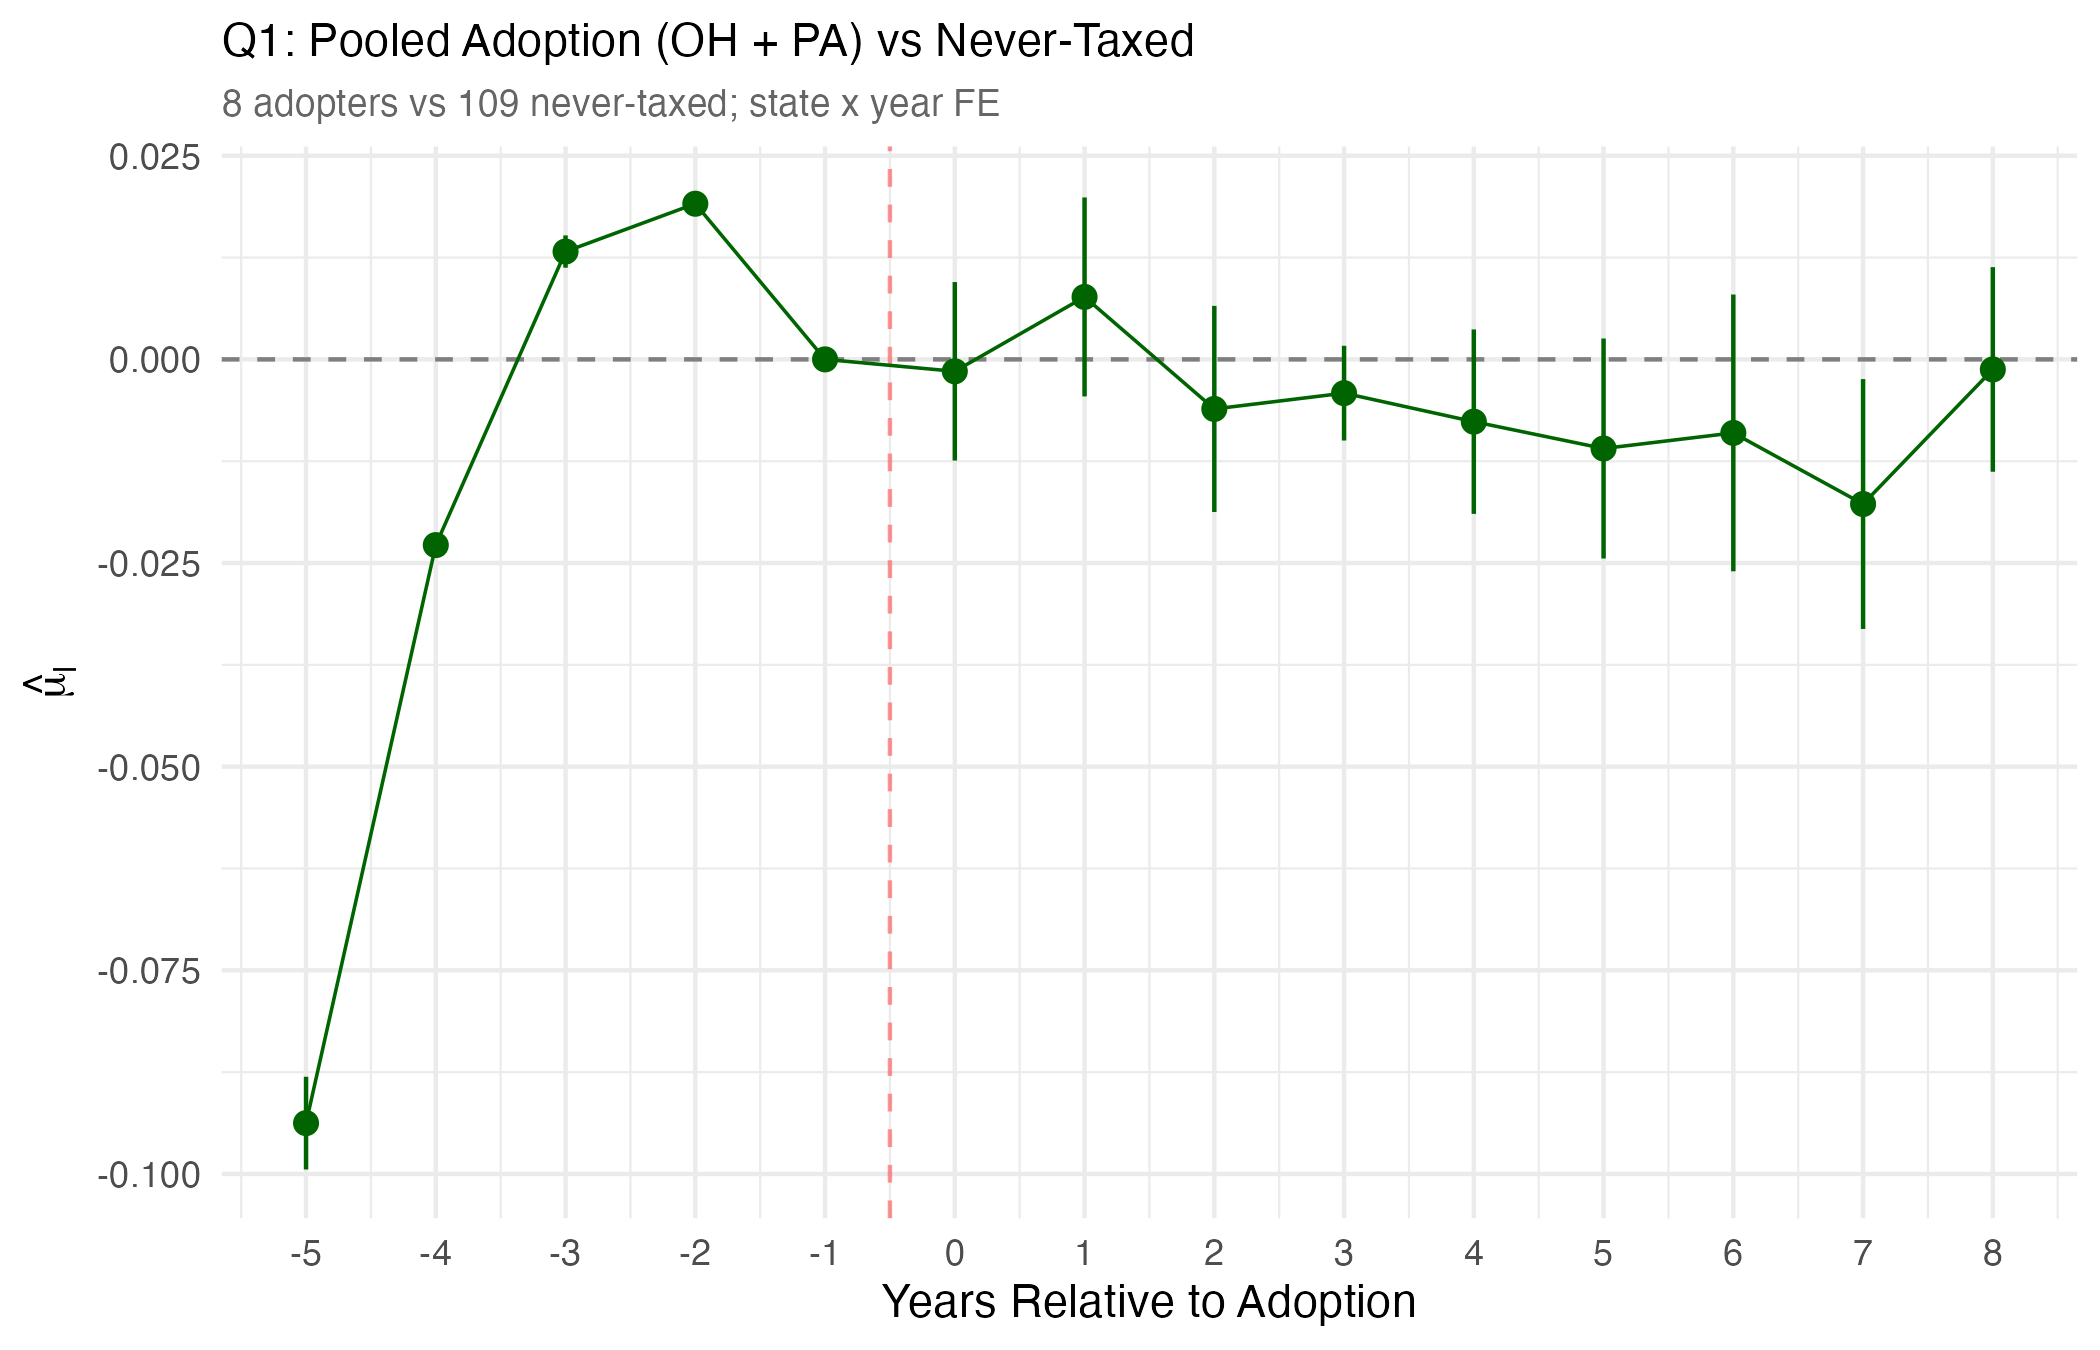
\includegraphics[width=0.85\textwidth]{../figures/q1_pooled_adoption.png}
    \caption{Q1: Pooled Adoption Event Study (OH + PA). 8 adopters vs
    109 never-taxed controls. State $\times$ year FE. Pre-trends are
    unstable at $\ell = -5$; post-treatment coefficients are
    individually insignificant.}
    \label{fig:q1}
\end{figure}

\textbf{A1:} We cannot reject the null. The pooled ATT is $-0.004$
(SE $0.007$), directionally consistent with sorting but statistically
insignificant. Only 8 municipalities adopted a tax during the panel
with sufficient LODES employment data, providing insufficient power
for the extensive margin. The effect size is small relative to the
intensive-margin results in Q2, though the comparison is imprecise.
We turn to rate \textit{changes} among already-taxed municipalities,
where sample sizes are substantially larger.


\subsection{Q2: Do Rate Increases Cause Sorting?}
\label{subsec:q2}

\begin{table}[H]
    \centering
    \caption{Q2: Effect of Rate Increases on share\_live\_in}
    \label{tab:q2}
    \small
    \begin{tabular}{lcccc}
        \toprule
        & \multicolumn{2}{c}{Inc vs No-Tax} & \multicolumn{2}{c}{Inc vs Stable-Rate} \\
        \cmidrule(lr){2-3} \cmidrule(lr){4-5}
        & (1) OH & (2) PA & (3) OH & (4) PA \\
        \midrule
        \multicolumn{5}{l}{\textit{Sun-Abraham (binary treatment)}} \\
        ATT                    & $-0.0074$\sym{**} & $-0.0091$\sym{.} & $-0.0001$         & $-0.0053$\sym{.} \\
                               & (0.0025)           & (0.0046)          & (0.0021)           & (0.0029)          \\[4pt]
        \multicolumn{5}{l}{\textit{DCDH (continuous treatment)}} \\
        Avg Total Effect       & $-0.2314$          & ---               & $0.0446$           & $-0.0078$         \\
                               & (0.3863)           &                   & (0.3132)           & (0.0069)          \\[2pt]
        Placebo $p$            & 0.406              & ---               & 0.147              & 0.904             \\
        \midrule
        Treated                & 252                & 157               & 252                & 196               \\
        Control                & 104 no-tax         & 5 no-tax          & 403 stable         & 2{,}209 stable    \\
        \bottomrule
    \end{tabular}
    \vspace{0.3em}
    \begin{minipage}{0.92\textwidth}
        \footnotesize \textit{Notes:} Columns organized by control group.
        ``No-tax'' = municipalities that never levied a local income
        tax. ``Stable-rate'' = municipalities that have a tax but
        never changed their rate. Sun-Abraham rows: binary treatment
        (1 after first rate increase). DCDH rows: continuous treatment
        (actual tax rate) via de Chaisemartin and D'Haultfoeuille (2024)
        with \texttt{continuous(1)}. PA DCDH vs no-tax omitted (only 5
        controls). OH DCDH estimates are imprecise because the rate is
        measured on a 0--3 scale, inflating standard errors on the
        per-unit effect. PA DCDH vs stable-rate has clean pre-trends
        (placebo $p = 0.90$).
        \sym{.}$p<0.10$, \sym{*}$p<0.05$, \sym{**}$p<0.01$, \sym{***}$p<0.001$.
    \end{minipage}
\end{table}

\begin{figure}[H]
    \centering
    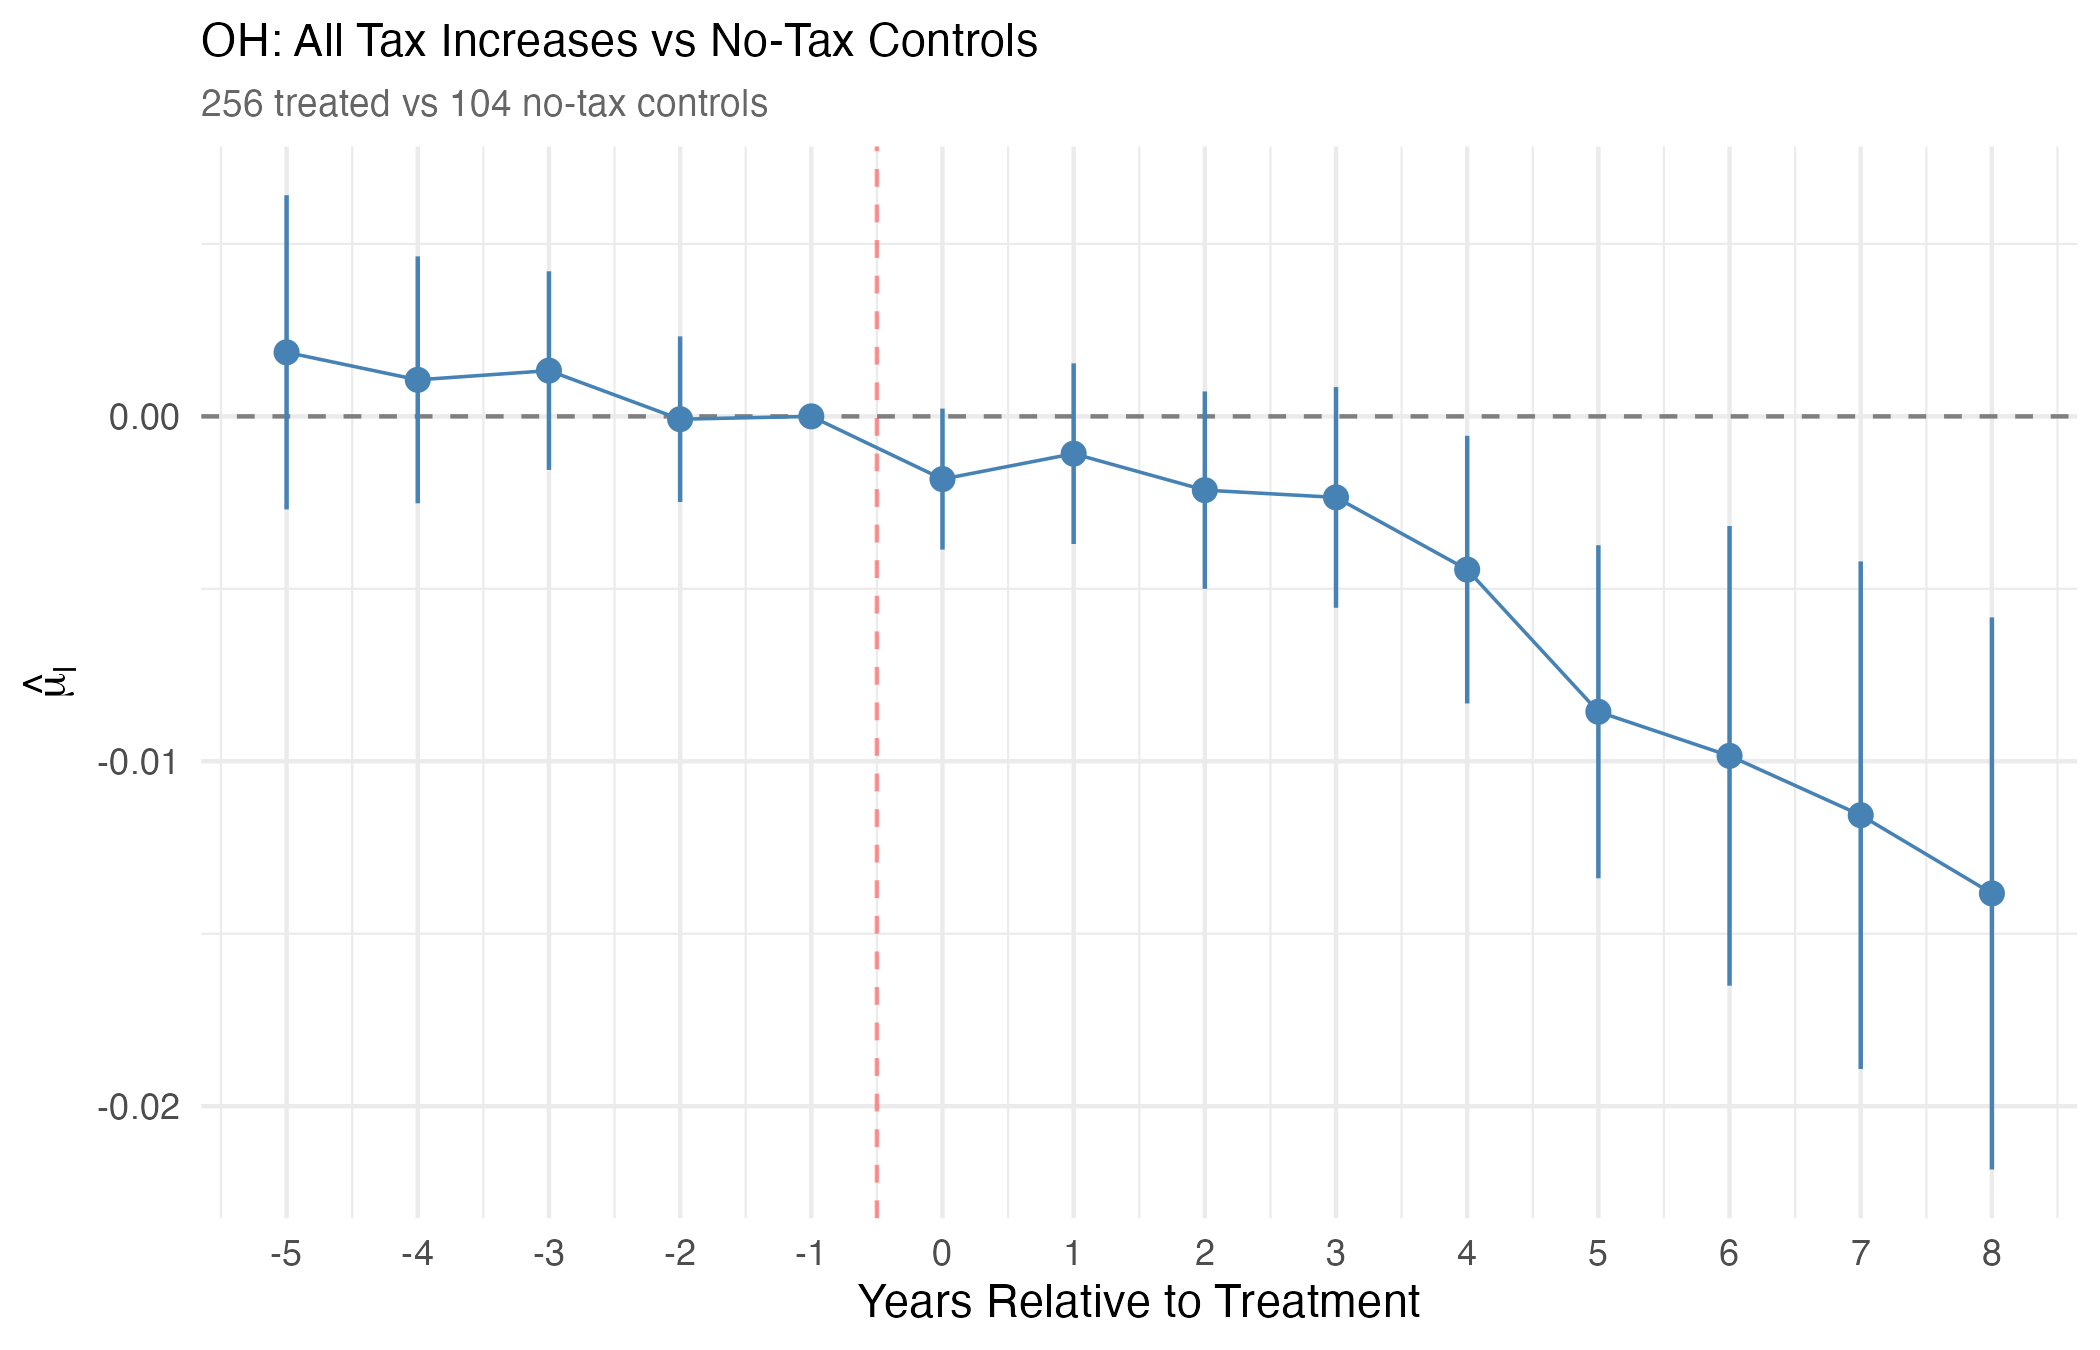
\includegraphics[width=0.85\textwidth]{../figures/q4_oh_all_inc.png}
    \caption{Q2 col (1): OH Rate Increases vs No-Tax Controls. Clean pre-trends; gradual decline through $t{+}8$.}
    \label{fig:q2_oh_notax}
\end{figure}

\begin{figure}[H]
    \centering
    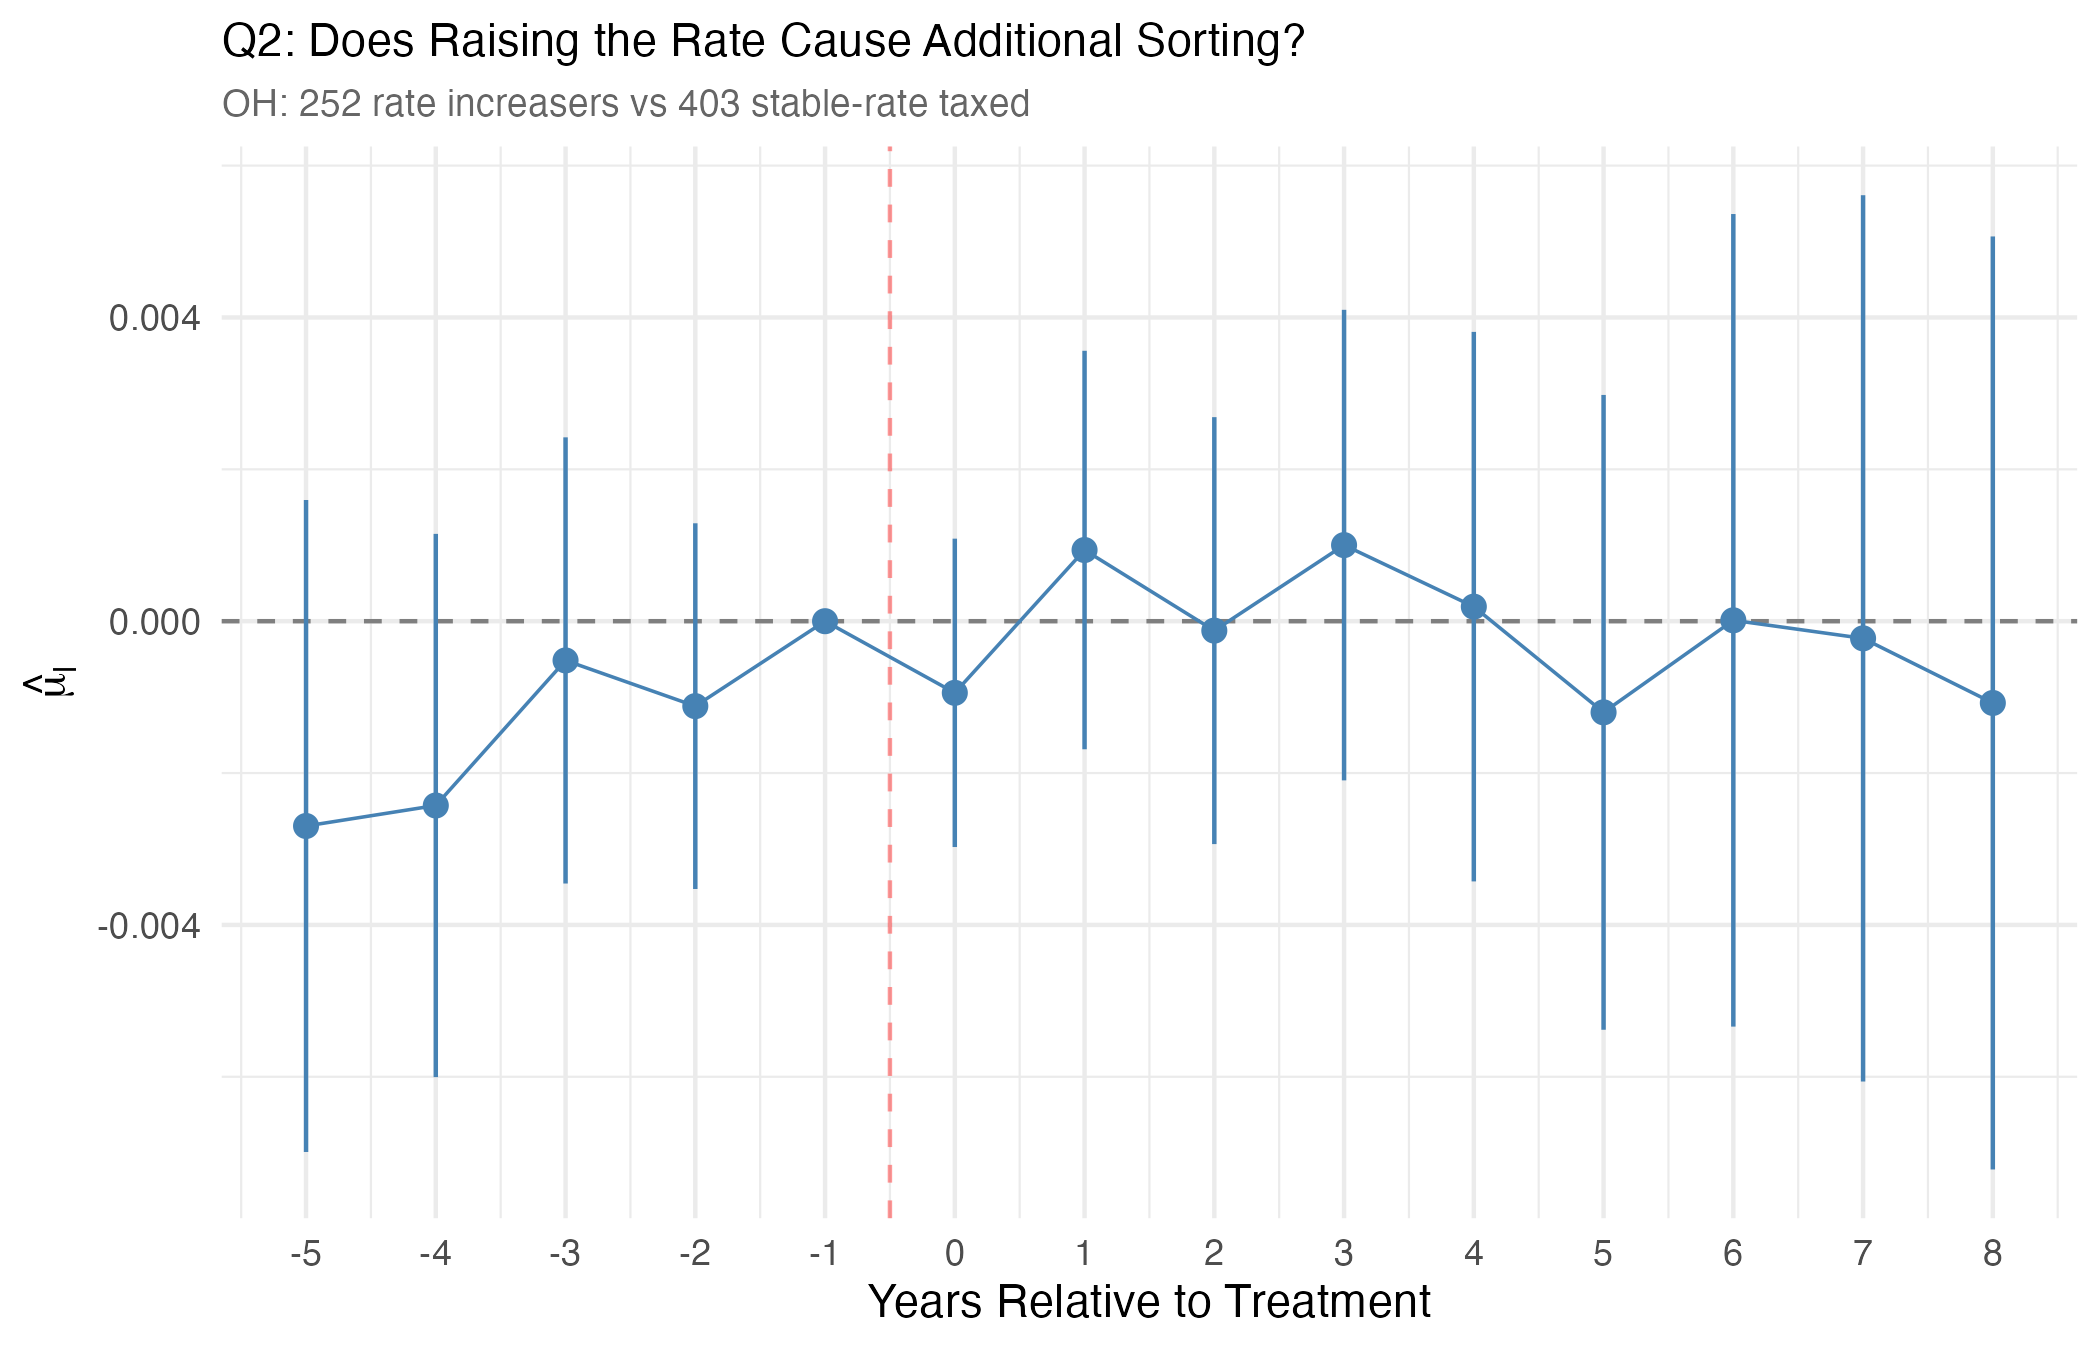
\includegraphics[width=0.85\textwidth]{../figures/q2_oh_intensive.png}
    \caption{Q2 col (2): OH Rate Increases vs Stable-Rate Taxed Cities. Null --- stable-rate cities are poor controls.}
    \label{fig:q2_oh}
\end{figure}

\begin{figure}[H]
    \centering
    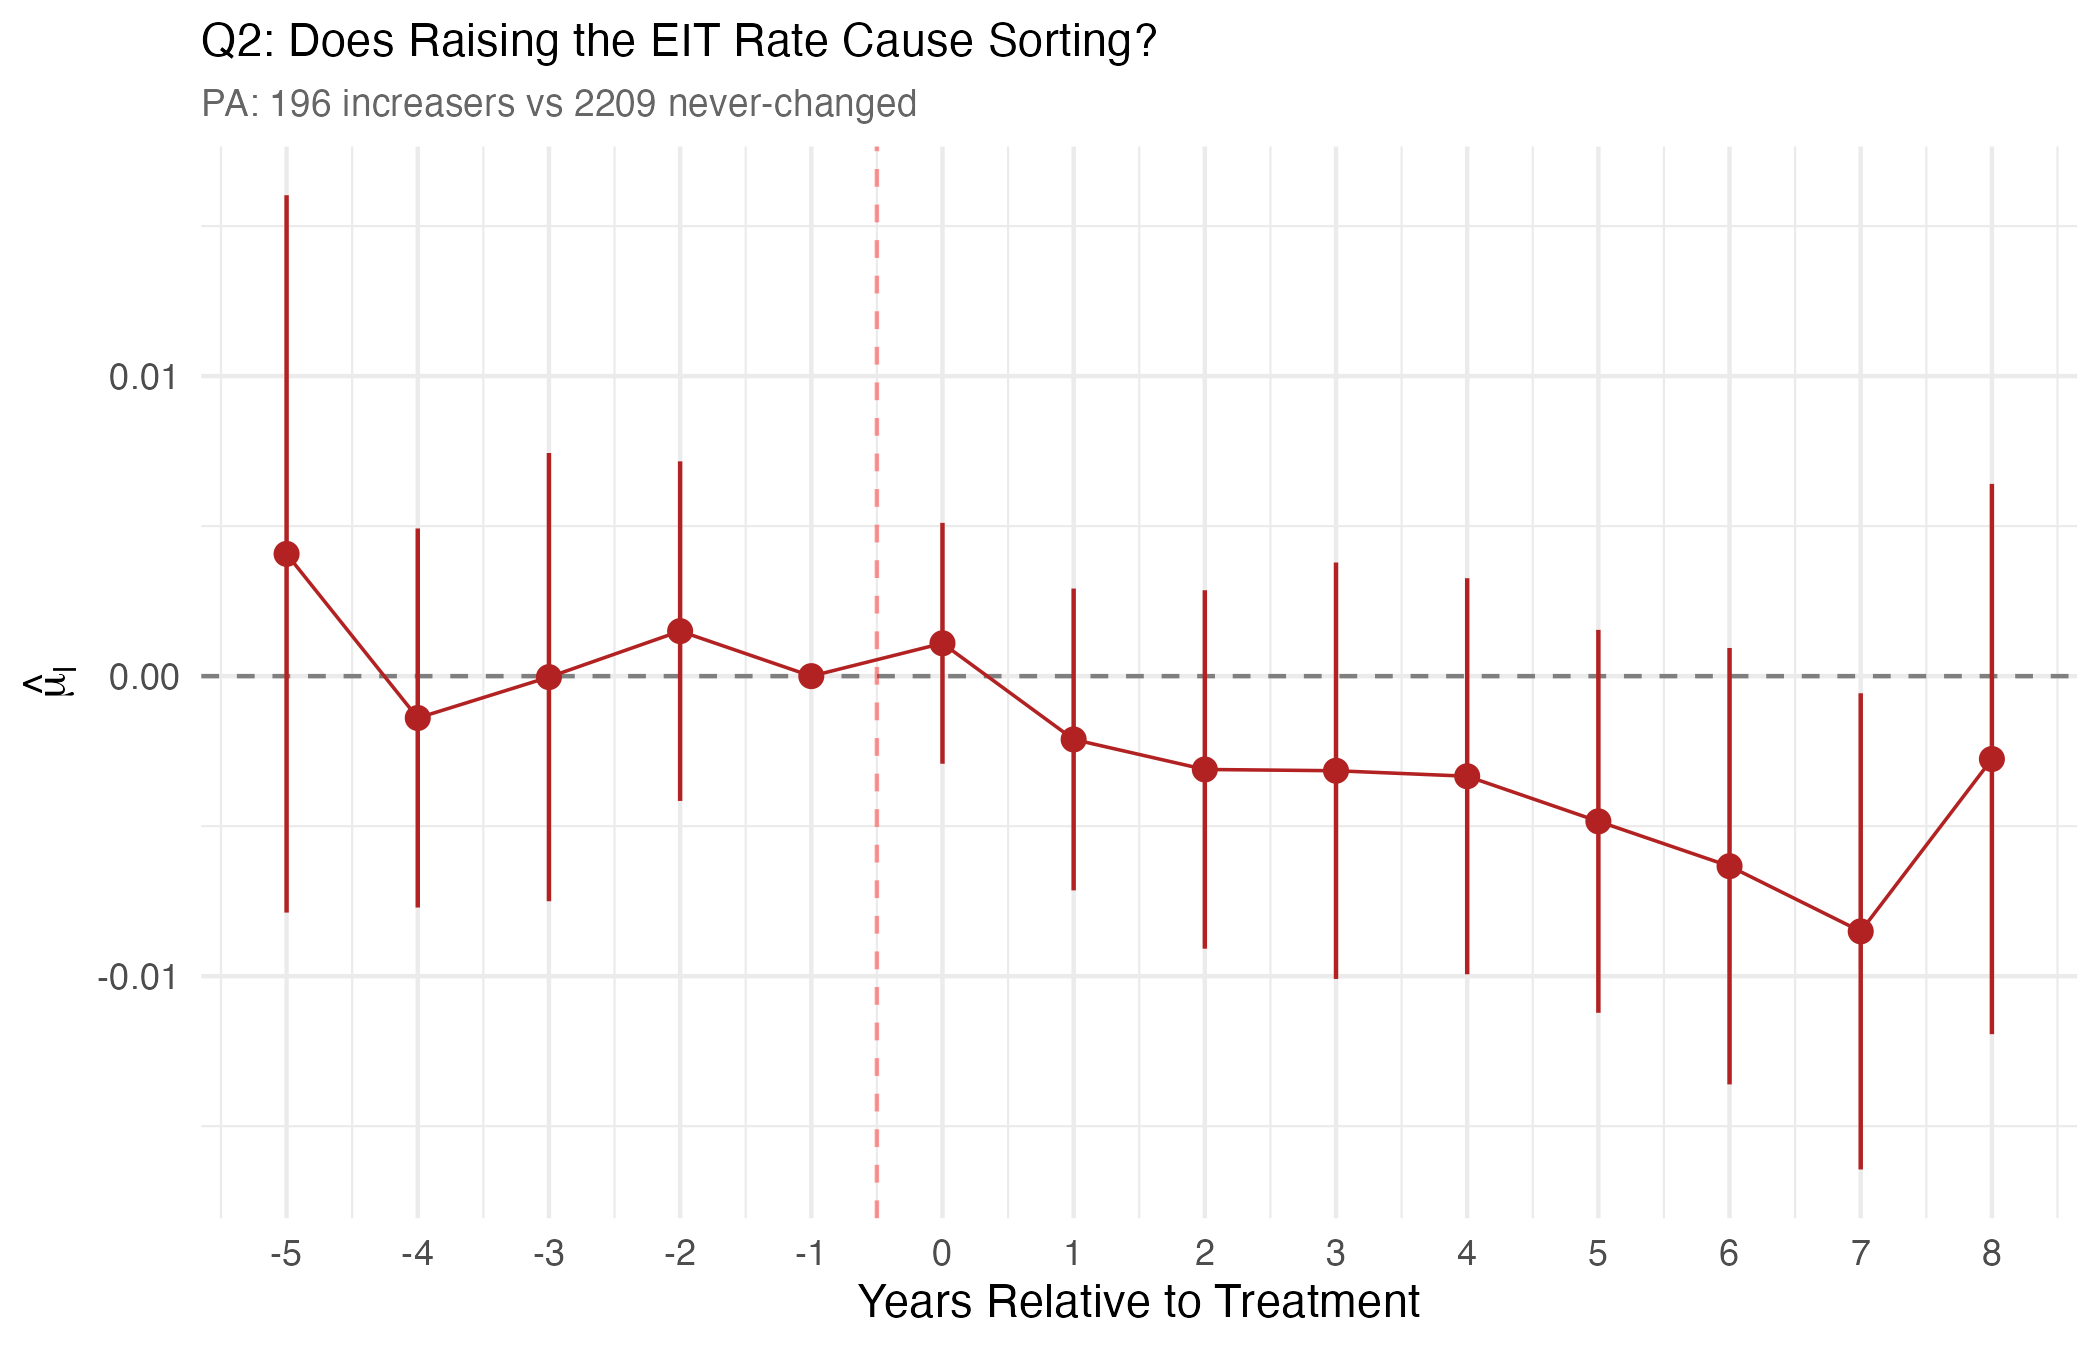
\includegraphics[width=0.85\textwidth]{../figures/q2_pa_intensive.png}
    \caption{Q2 col (3): PA Rate Increases vs Stable-Rate Municipalities.}
    \label{fig:q2_pa}
\end{figure}

\begin{figure}[H]
    \centering
    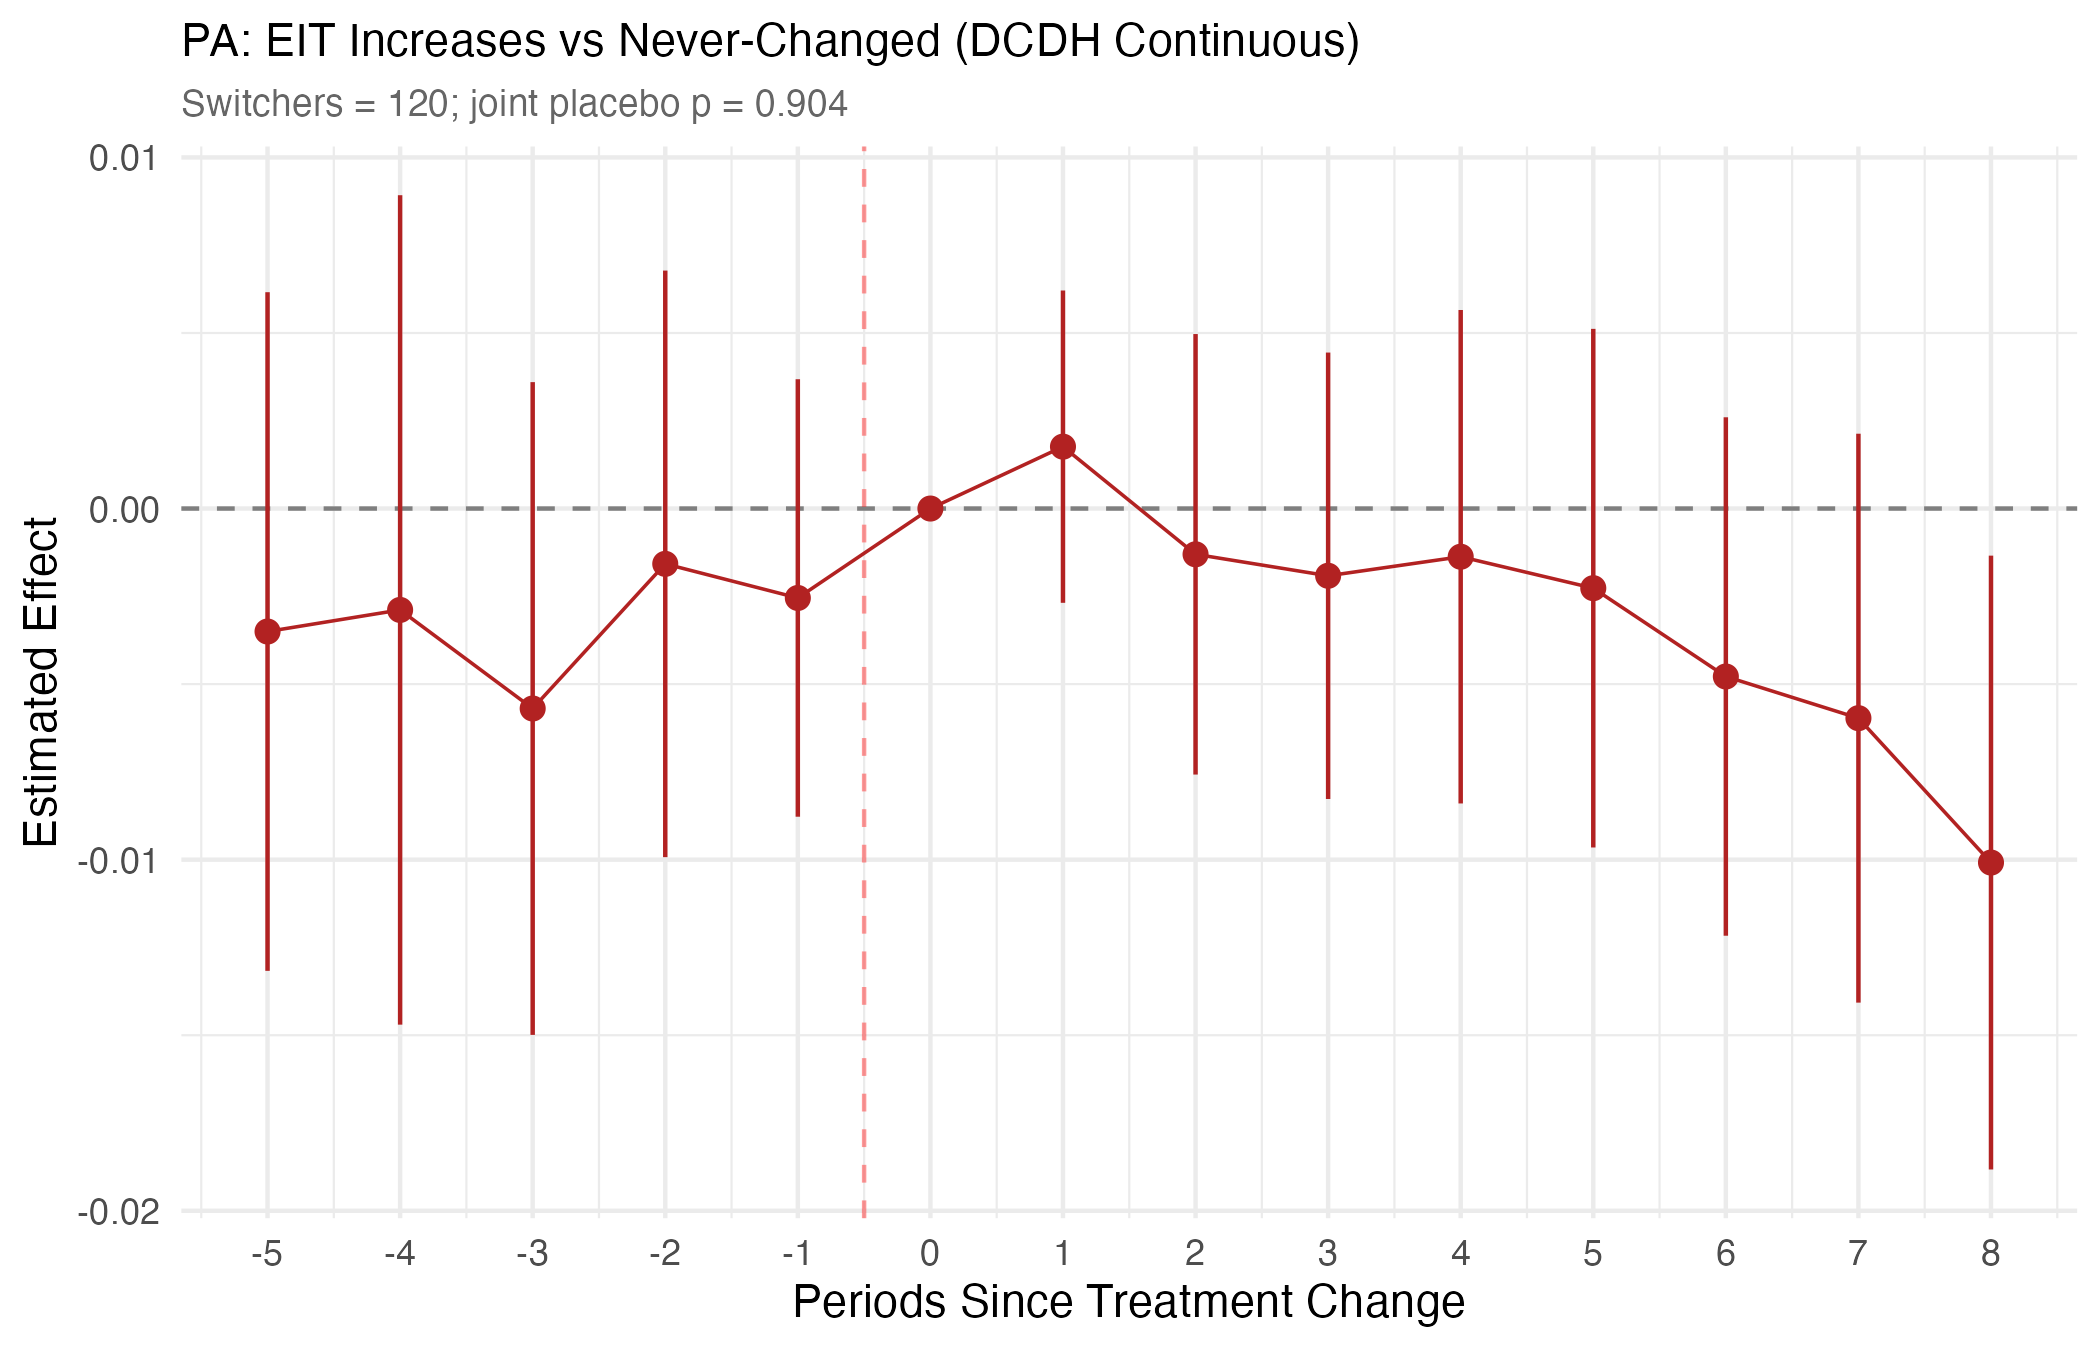
\includegraphics[width=0.85\textwidth]{../figures/pa_dcdh_inc.png}
    \caption{Q2 col (4): PA DCDH Continuous EIT Rate. Clean pre-trends (placebo $p = 0.90$); effect reaches $-0.011^{***}$ at $\ell = 8$.}
    \label{fig:q2_pa_dcdh}
\end{figure}

\textbf{A2:} Yes. Rate increases reduce the locally-resident worker
share. The effect is $-0.005$ to $-0.008$ per percentage point and
builds gradually over 7--8 years. The result is robust across
estimators (Sun-Abraham binary and DCDH continuous) and both states.
The choice of control group matters for Ohio: no-tax townships produce
a significant effect ($-0.007^{**}$) while stable-rate taxed cities
produce a null, suggesting that the latter share confounding urban
characteristics with treated cities.


\subsection{Q3: Do Rate Decreases Reverse Sorting?}
\label{subsec:q3}

\begin{table}[H]
    \centering
    \caption{Q3: Effect of Rate Decreases on share\_live\_in}
    \label{tab:q3}
    \small
    \begin{tabular}{lccc}
        \toprule
        & (1) & (2) & (3) \\
        & PA: Dec vs & PA: Dec & OH: Dec vs \\
        & Stable-Rate & DCDH & No-Tax \\
        \midrule
        Sun-Abraham ATT        & $0.0048$     &              & $-0.0042$    \\
                               & (0.0057)     &              & (0.0064)     \\[3pt]
        DCDH Avg Total Effect  &              & $-0.0077$    &              \\
                               &              & (0.0090)     &              \\
        \midrule
        Treated / Switchers    & 94           & 60           & 36           \\
        Control                & 2{,}209 NC   & NC           & 104 no-tax   \\
        Placebo $p$            & ---          & 0.408        & ---          \\
        \bottomrule
    \end{tabular}
    \vspace{0.3em}
    \begin{minipage}{0.85\textwidth}
        \footnotesize \textit{Notes:} Column (1): PA Sun-Abraham ATT for
        decreasers vs stable-rate municipalities (null). Column (2): PA
        DCDH continuous among decreasers (negative ATE --- decreases do
        not increase share\_live\_in). Column (3): OH decreasers vs
        no-tax townships (null, 36 treated).
        \sym{.}$p<0.10$, \sym{*}$p<0.05$, \sym{**}$p<0.01$, \sym{***}$p<0.001$.
    \end{minipage}
\end{table}

\begin{figure}[H]
    \centering
    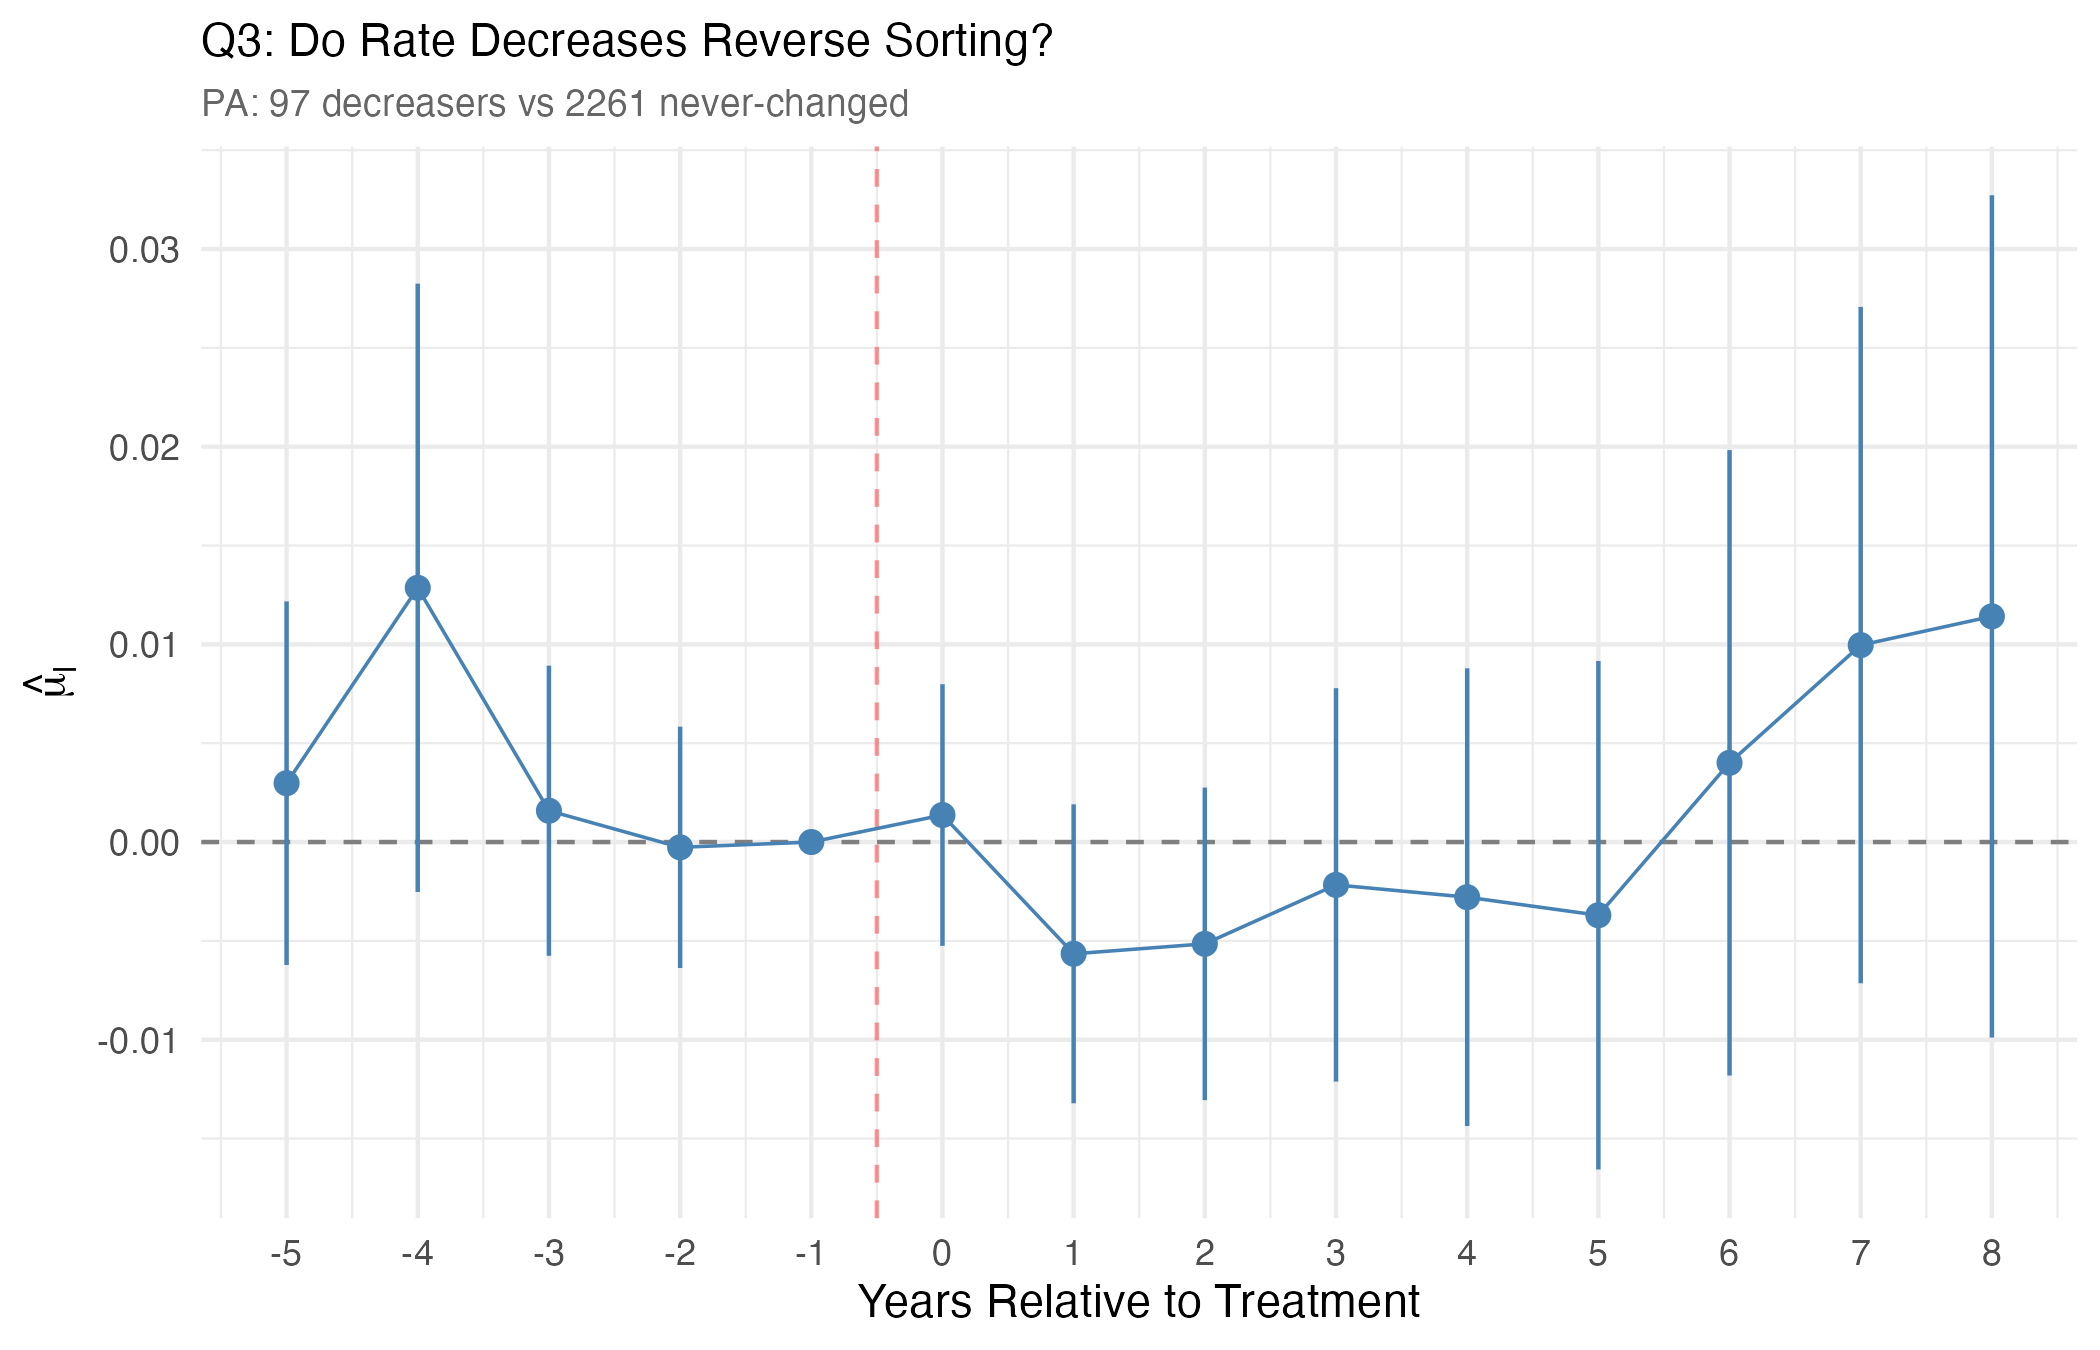
\includegraphics[width=0.85\textwidth]{../figures/q3_pa_decrease.png}
    \caption{Q3 col (1): PA Rate Decreases vs Stable-Rate. No evidence of reversal.}
    \label{fig:q3_pa}
\end{figure}

\begin{figure}[H]
    \centering
    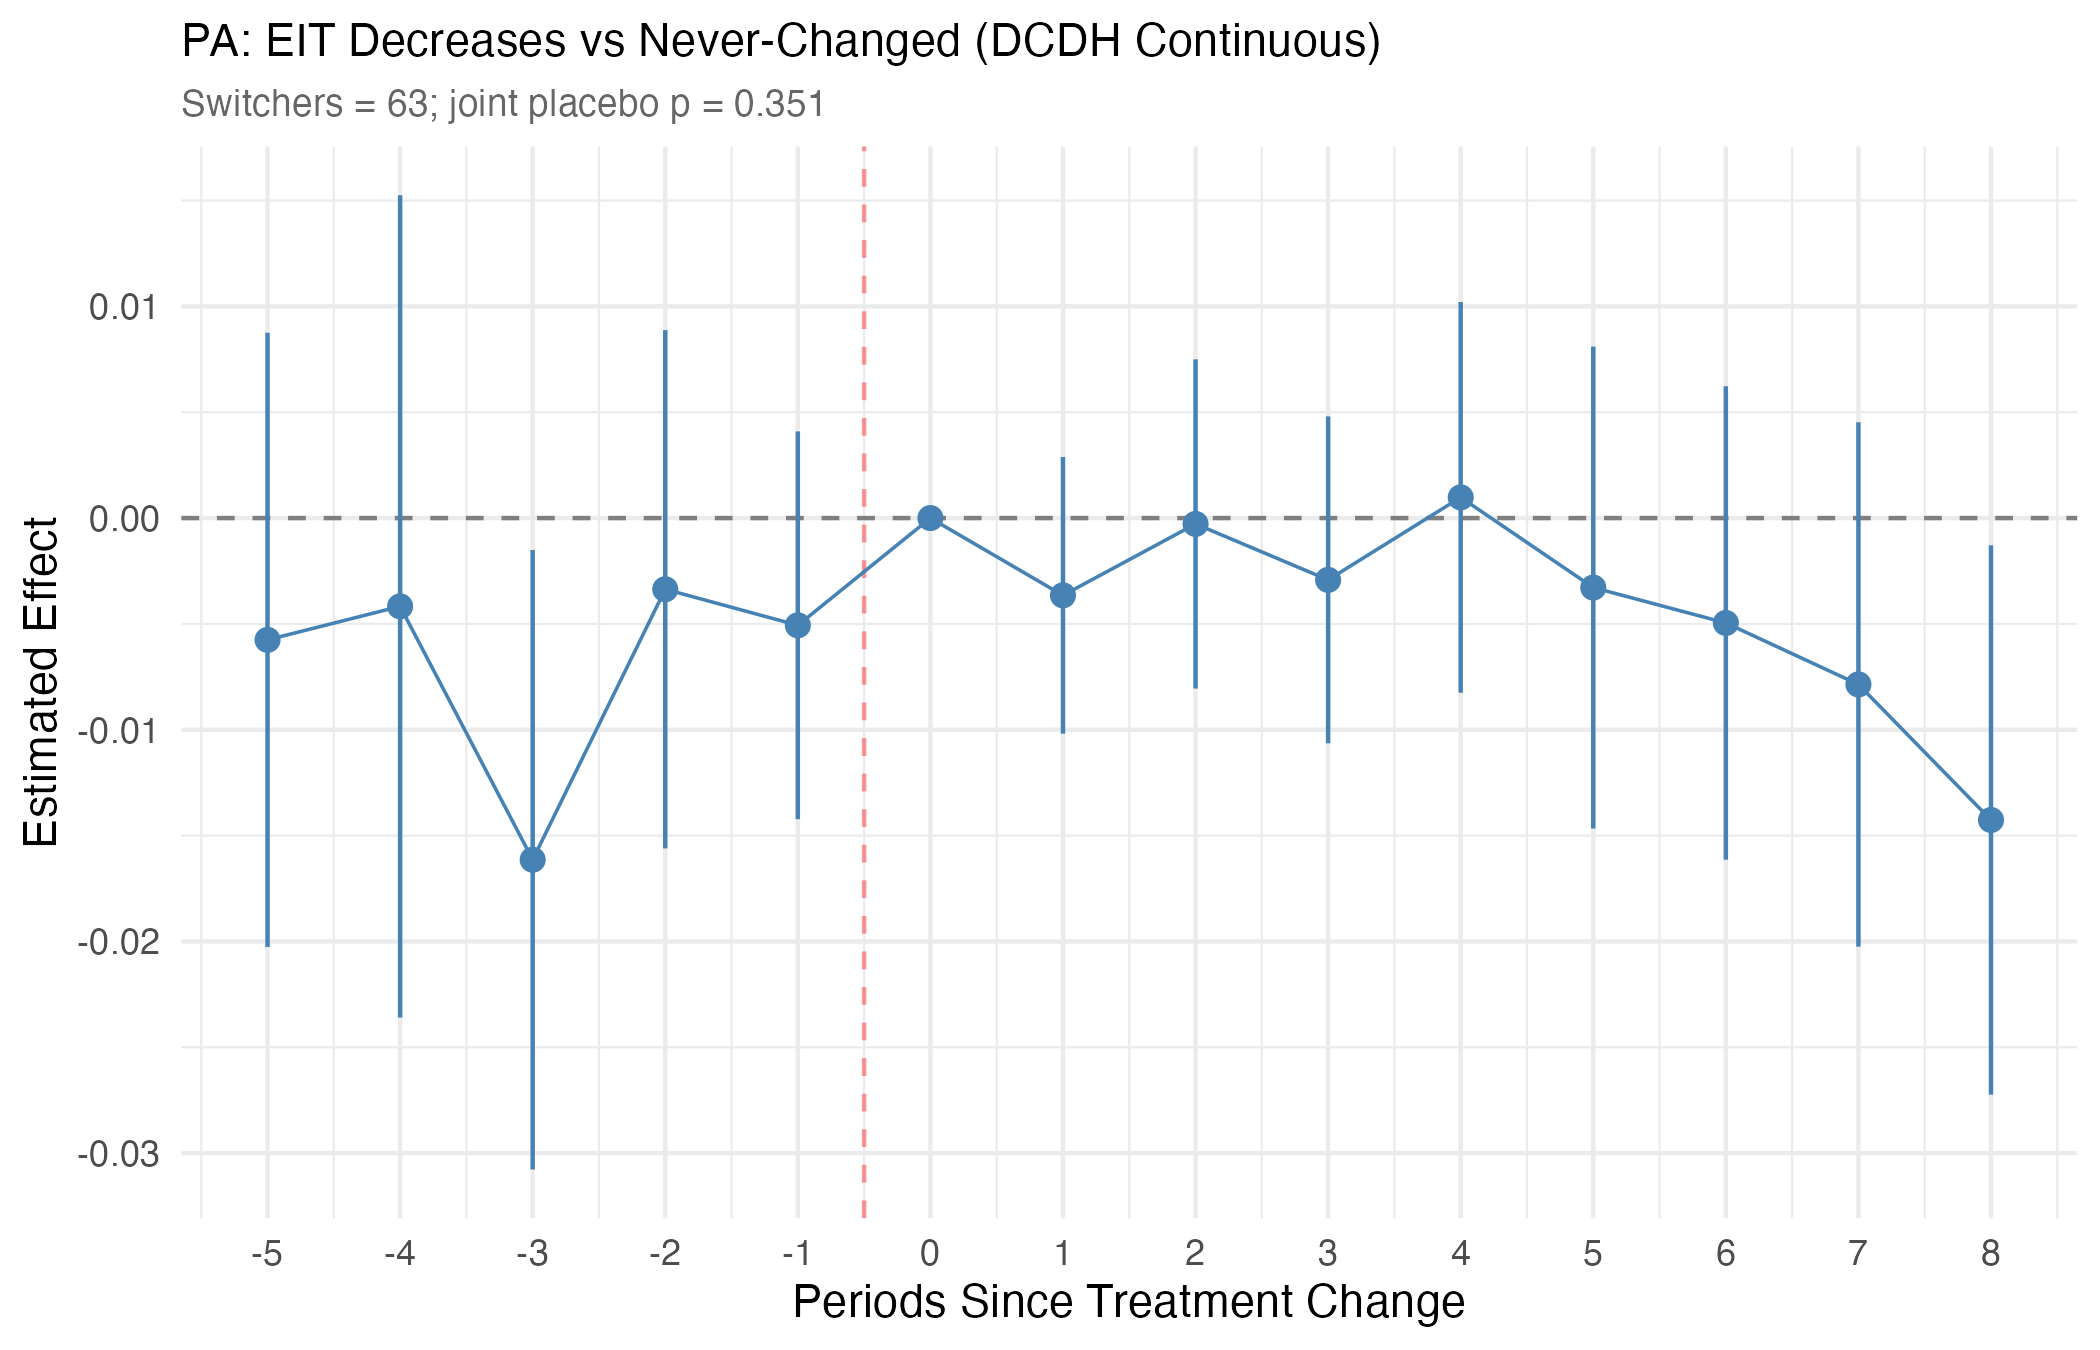
\includegraphics[width=0.85\textwidth]{../figures/pa_dcdh_dec.png}
    \caption{Q3 col (2): PA DCDH Continuous, Decreasers vs Stable-Rate.}
    \label{fig:q3_pa_dcdh}
\end{figure}

\begin{figure}[H]
    \centering
    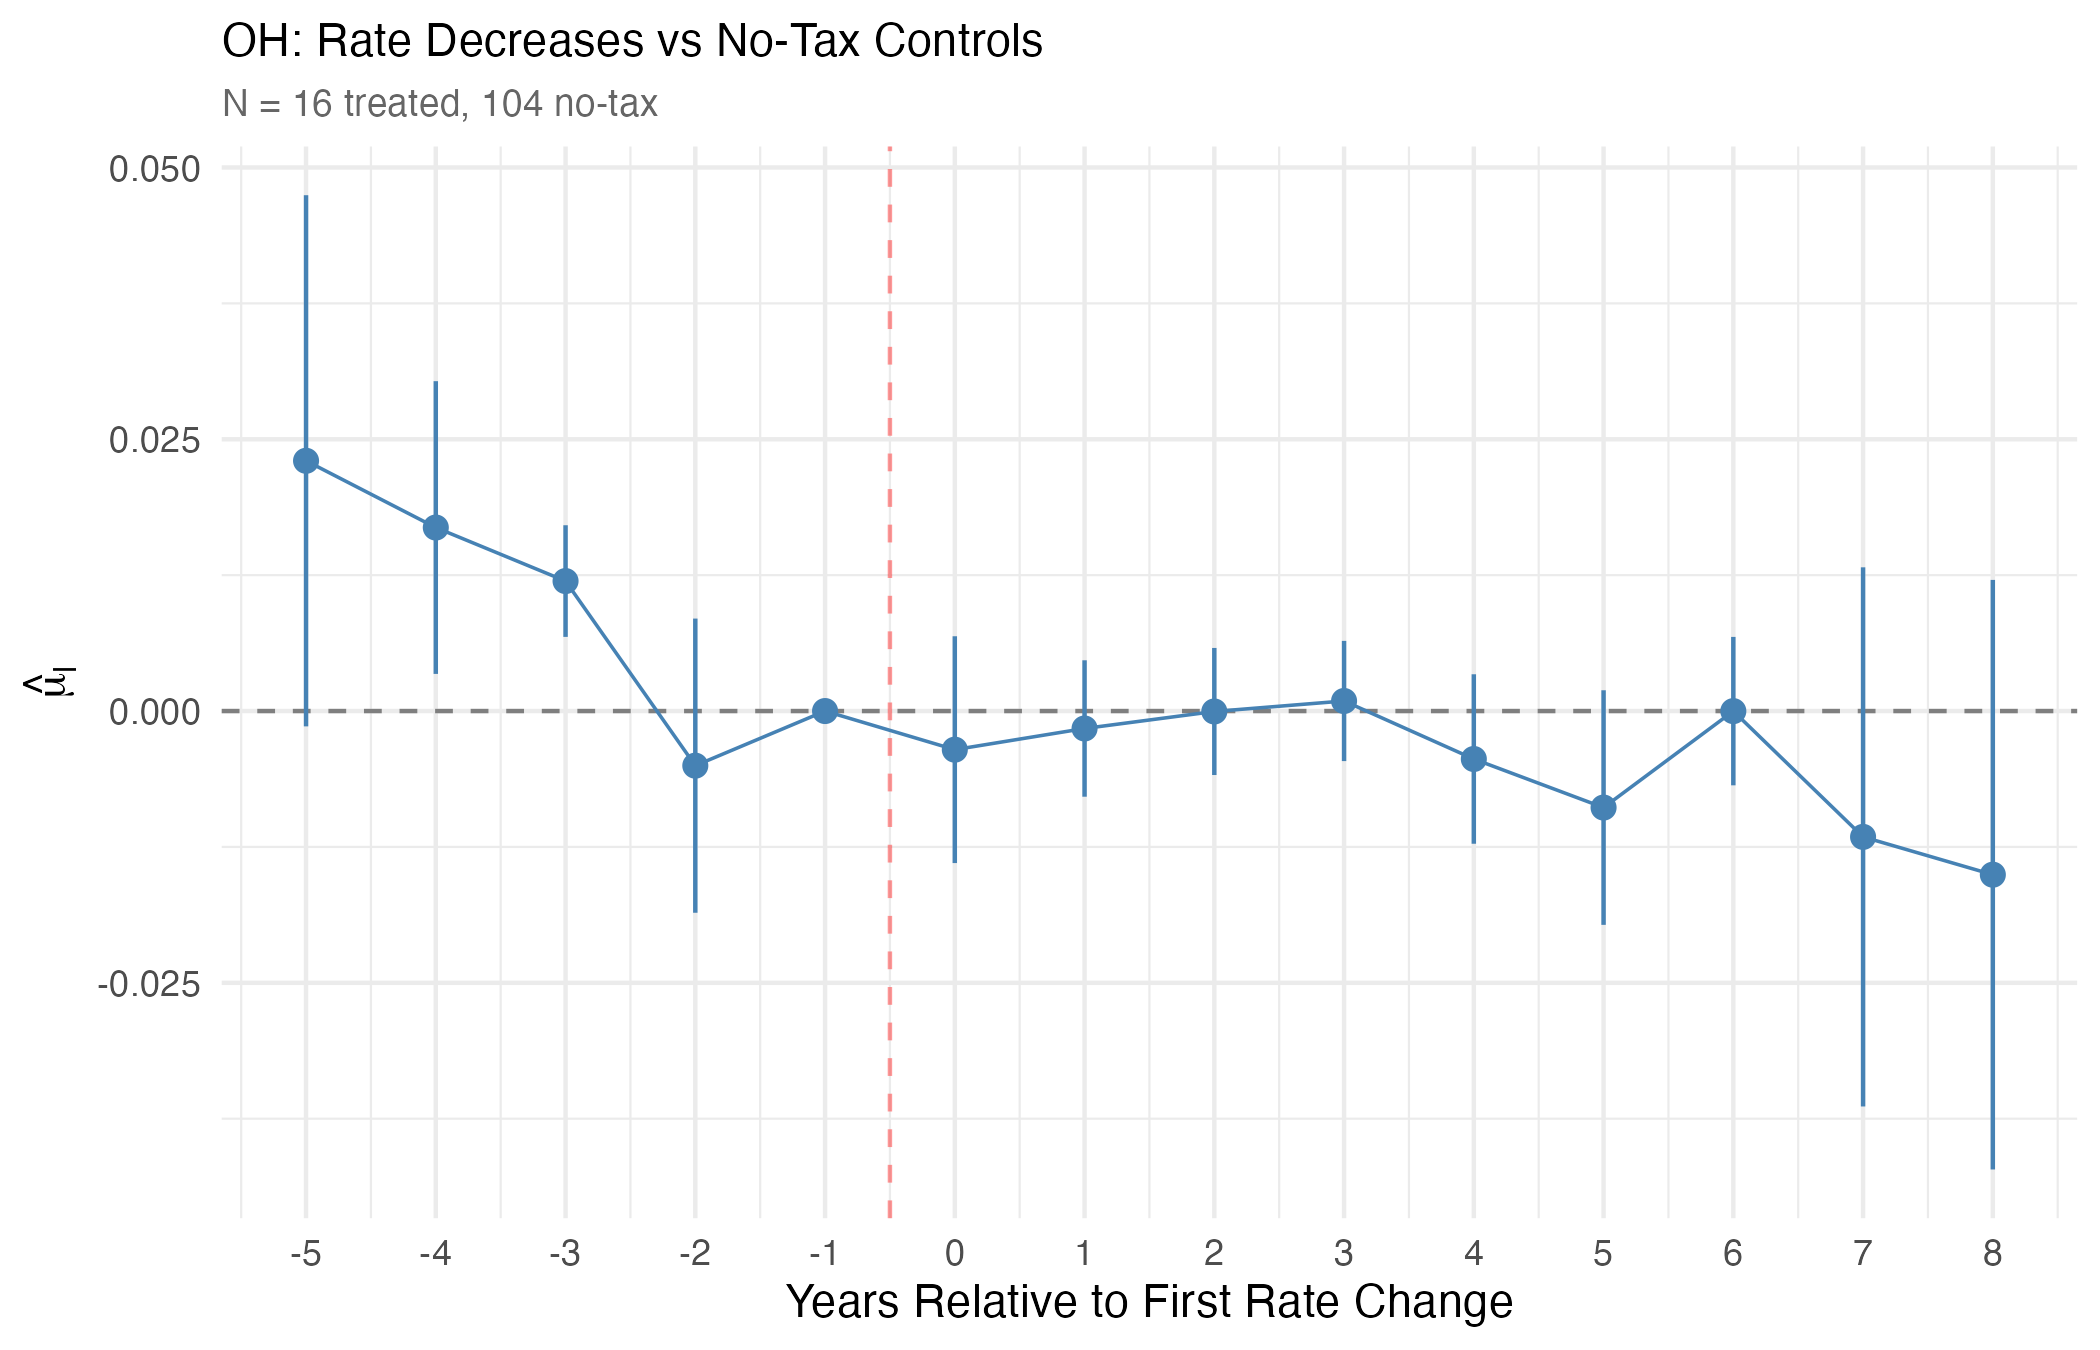
\includegraphics[width=0.85\textwidth]{../figures/oh_es_decrease_notax.png}
    \caption{Q3 col (3): OH Rate Decreases vs No-Tax. Wide confidence intervals.}
    \label{fig:q3_oh}
\end{figure}

\textbf{A3:} No. Rate decreases do not reverse sorting. All decrease
estimates are statistically indistinguishable from zero in both states.
The PA DCDH estimate is actually negative ($-0.008$), suggesting that
municipalities that cut their rates continue to lose locally-resident
workers, possibly because rate cuts signal fiscal distress.


\subsection{Q4: Is the Response Asymmetric?}
\label{subsec:q4}

\begin{table}[H]
    \centering
    \caption{Q4: Asymmetry Test --- Joint Increases and Decreases}
    \label{tab:q4}
    \small
    \begin{tabular}{lcccc}
        \toprule
        & \multicolumn{2}{c}{Pennsylvania} & \multicolumn{2}{c}{Ohio} \\
        \cmidrule(lr){2-3} \cmidrule(lr){4-5}
        & (1) & (2) & (3) & (4) \\
        & Joint Model & Split Dose & Joint Model & Split Dose \\
        \midrule
        inc $\times$ post      & $-0.0074$\sym{*} &              & $-0.0055$\sym{**} &              \\
                               & (0.0037)          &              & (0.0020)            &              \\[3pt]
        dec $\times$ post      & $-0.0002$         &              & $-0.0080$           &              \\
                               & (0.0060)          &              & (0.0126)            &              \\[3pt]
        $R^{+}$ (cum.\ inc)    &                   & $-0.0177$\sym{*} &               & $-0.109$     \\
                               &                   & (0.0069)     &                   & (0.379)      \\[3pt]
        $R^{-}$ (cum.\ dec)    &                   & $0.0012$     &                   & $-1.155$     \\
                               &                   & (0.0040)     &                   & (1.353)      \\
        \midrule
        $N$                    & 24{,}526          & 24{,}526     & 5{,}081           & 7{,}718      \\
        \bottomrule
    \end{tabular}
    \vspace{0.3em}
    \begin{minipage}{0.92\textwidth}
        \footnotesize \textit{Notes:} Columns (1), (3): joint model with
        increase and decrease post indicators. Columns (2), (4): split
        cumulative dose on full sample. PA: rate increases reduce
        share\_live\_in ($\beta^{+} = -0.018^{*}$ per pp); rate decreases
        have no effect ($\beta^{-} \approx 0$). OH split dose is
        imprecise (0--3 rate scale).
        \sym{.}$p<0.10$, \sym{*}$p<0.05$, \sym{**}$p<0.01$, \sym{***}$p<0.001$.
    \end{minipage}
\end{table}

\textbf{A4:} Yes, the response is asymmetric. Rate increases reduce
the locally-resident share ($\delta^{+} = -0.007^{*}$ in PA,
$-0.006^{**}$ in OH; $\beta^{+} = -0.018^{*}$ per pp in the split
dose), but rate decreases have no effect ($\delta^{-} \approx 0$,
$\beta^{-} \approx 0$). This pattern is consistent across both states,
both estimators (joint model and split dose), and the DCDH results
from Q3. Residential location decisions are sticky: once a tax
increase pushes workers to relocate their residence outside the
taxing municipality, cutting the rate does not bring them back.


\subsection{Companion Outcomes: Decomposition}
\label{subsec:decomposition}

% TODO: Framing: "A decline in share_live_in could reflect residential sorting,
% compositional change in the workforce, or differential job growth among
% nonresident commuters. To decompose the mechanism, we estimate the dose-response
% specification separately for the numerator (resident workers), denominator
% (total jobs), and nonresident commuters."
%
% Key finding: resident workers fall most, but total jobs also decline.
% Cannot reject equality of resident vs nonresident coefficients (p = 0.09).
% "The larger decline in resident workers is suggestive of a sorting channel,
% though the estimates also indicate broader employment effects."

% --- Companion Outcomes Table ---
\begin{table}[H]
    \centering
    \caption{Companion Outcomes: Decomposing the share\_live\_in Effect}
    \label{tab:companion}
    \small
    \begin{tabular}{lcccc}
        \toprule
        & (1) & (2) & (3) & (4) \\
        & share\_live\_in & log(Resident) & log(Nonresident) & log(Total Jobs) \\
        \midrule
        \multicolumn{5}{l}{\textit{PA Dose-Response (treated municipalities only)}} \\
        rate $\times$ post     & $-0.0099^{.}$  & $-0.1530^{*}$  & $-0.1012^{.}$  & $-0.1172^{*}$  \\
                               & (0.0052)       & (0.0720)       & (0.0548)       & (0.0549)       \\[3pt]
        post                   & 0.0022         & $0.1226^{.}$   & $0.1113^{.}$   & $0.1173^{*}$   \\
                               & (0.0064)       & (0.0721)       & (0.0596)       & (0.0587)       \\
        \midrule
        \multicolumn{5}{l}{\textit{Diagnostics}} \\
        N                      & 2{,}741        & 2{,}741        & 2{,}741        & 2{,}741        \\
        $R^2$                  & 0.912          & 0.979          & 0.980          & 0.982          \\
        Within $R^2$           & 0.011          & 0.015          & 0.008          & 0.011          \\
        Fixed Effects          & \multicolumn{4}{c}{Municipality, Year} \\
        Clusters               & \multicolumn{4}{c}{Municipality} \\
        Equality test (2) vs (3) & \multicolumn{4}{c}{$p = 0.09$} \\
        \bottomrule
    \end{tabular}
    \vspace{0.3em}
    \begin{minipage}{0.85\textwidth}
        \footnotesize \textit{Notes:} Dose-response specification estimated among PA
        municipalities that raised EIT rates, 2002--2019. Column (1): main outcome.
        Columns (2)--(4): log counts of resident workers (live and work in municipality),
        nonresident commuters (work in municipality, live elsewhere), and total jobs.
        Equality test: joint model testing whether the resident coefficient differs from
        the nonresident coefficient.
        $^{.}p<0.10$, $^{*}p<0.05$, $^{**}p<0.01$, $^{***}p<0.001$.
    \end{minipage}
\end{table}

\begin{figure}[H]
    \centering
    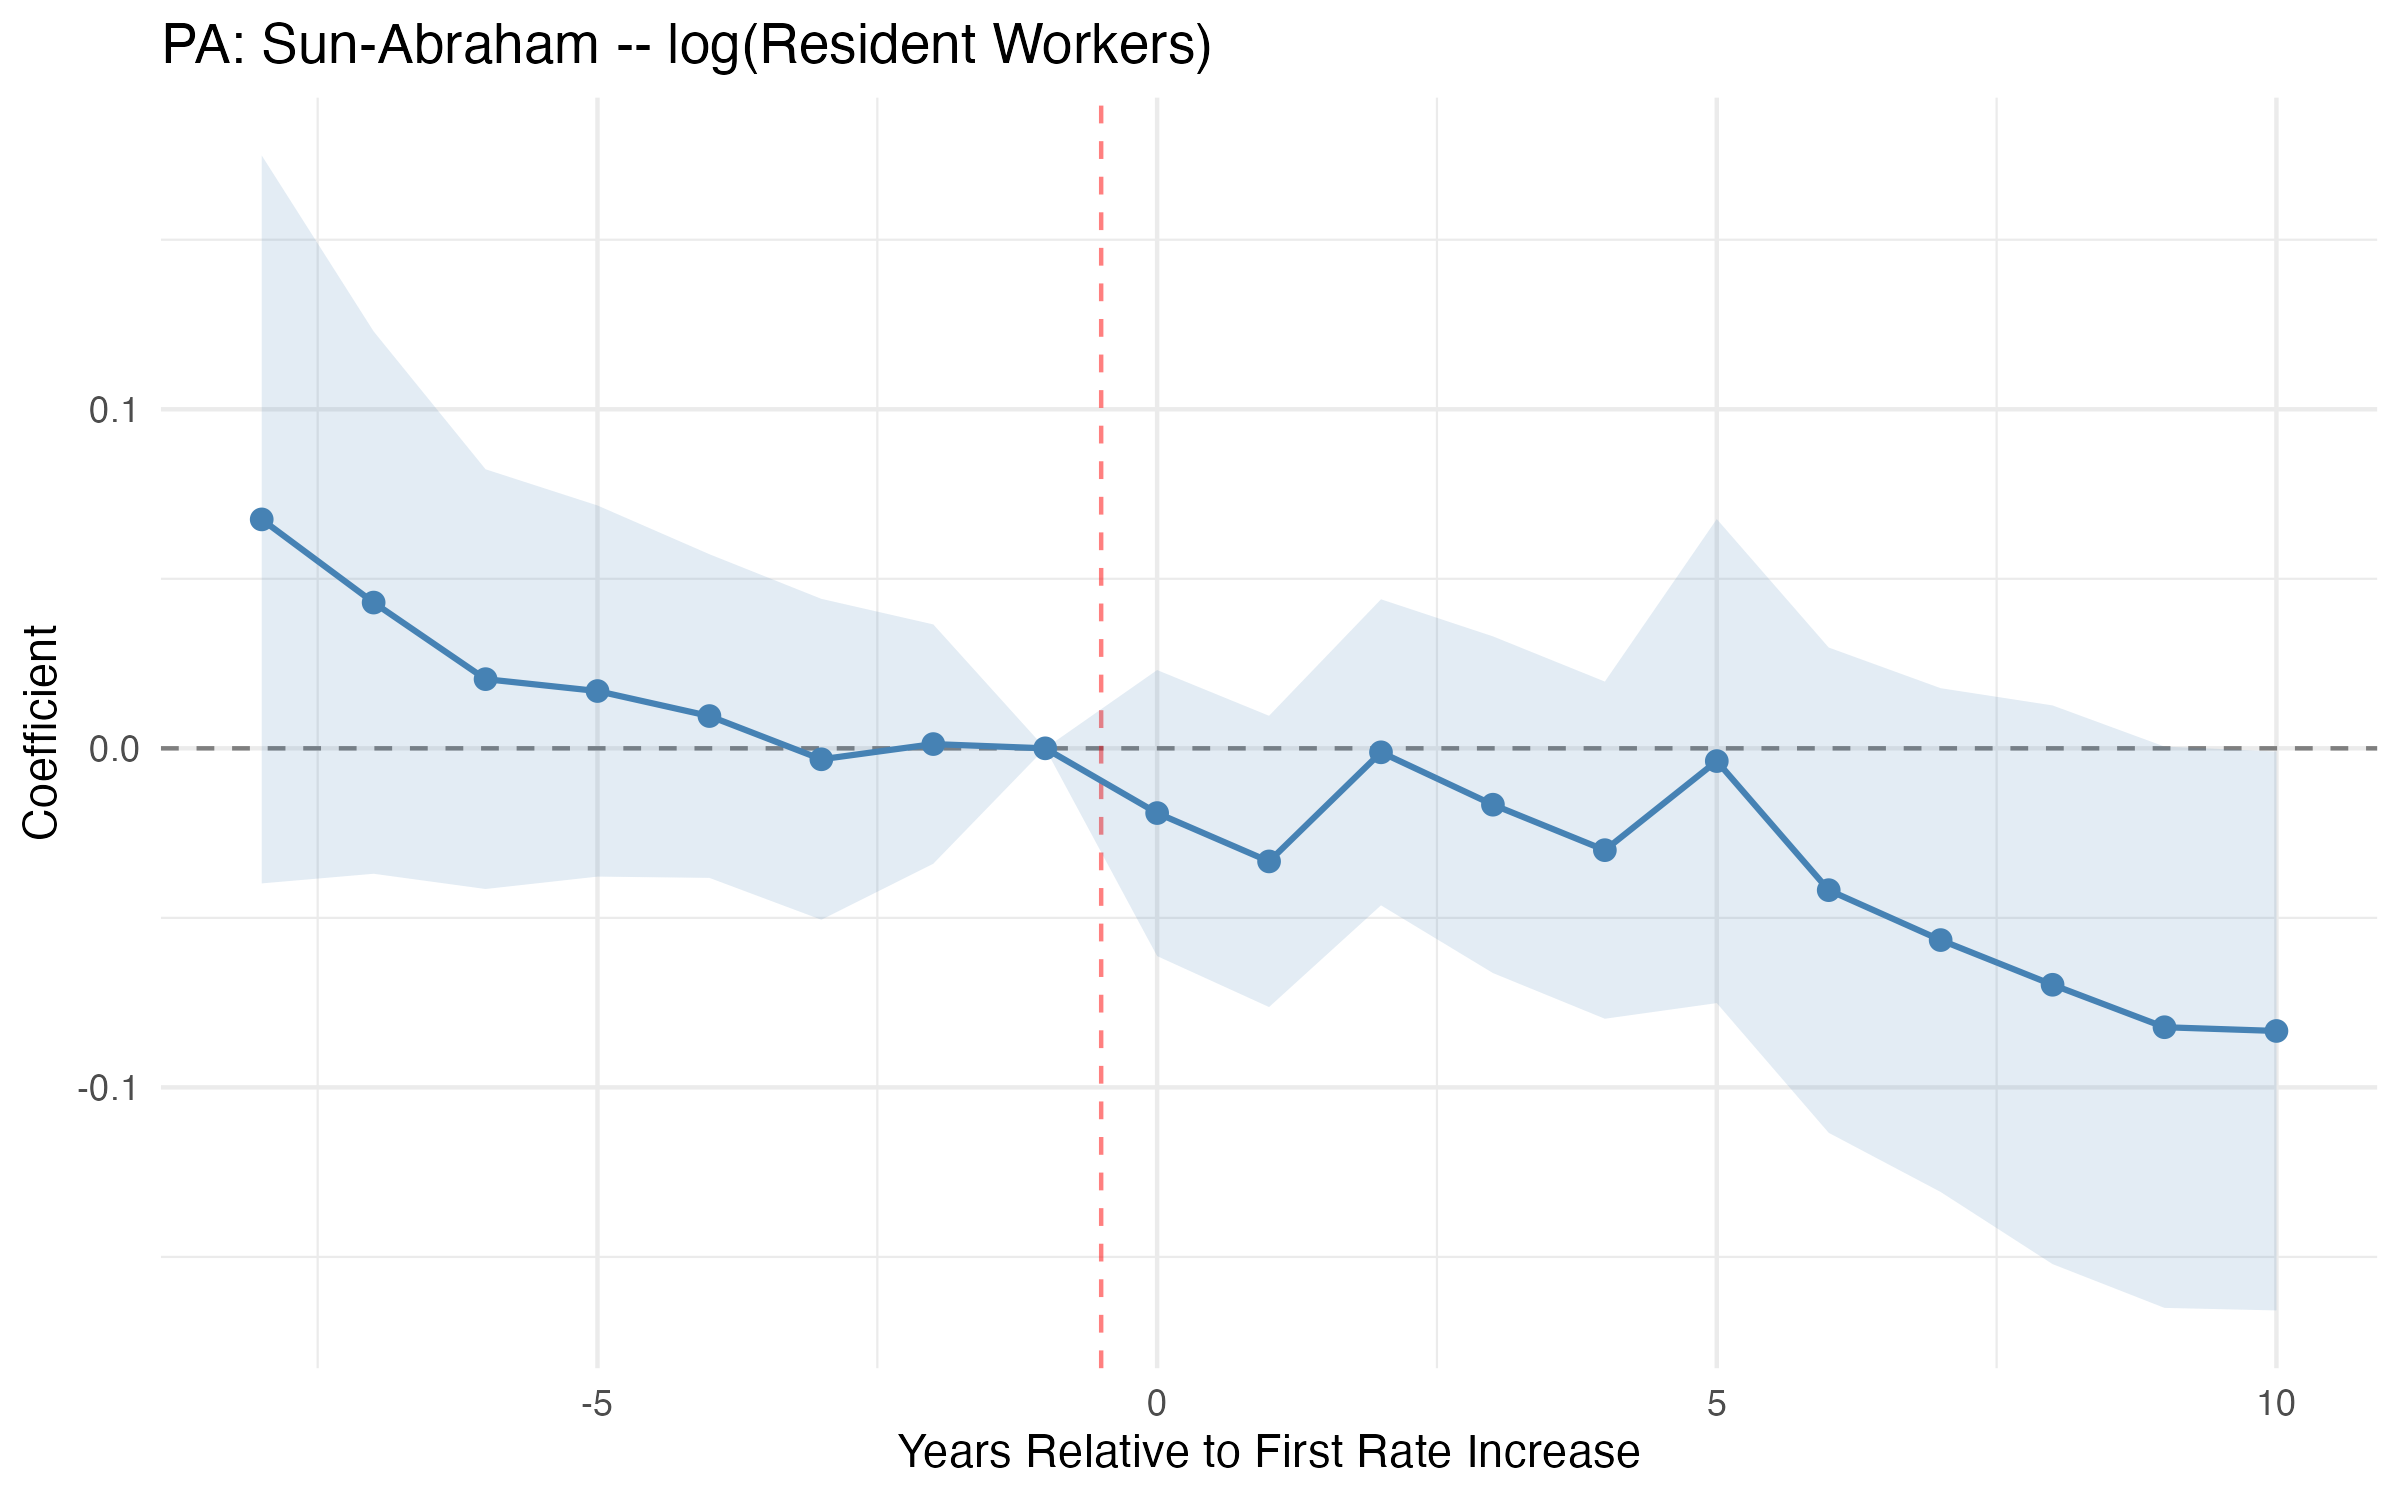
\includegraphics[width=0.85\textwidth]{../figures/pa_sunab_resident.png}
    \caption{Pennsylvania: Sun-Abraham Event Study --- log(Resident Workers).}
    \label{fig:pa_sunab_resident}
\end{figure}

\subsection{Fiscal Impact}
\label{subsec:fiscal}

% TODO: "Using PA DCED Annual Financial Reports, we estimate the fiscal
% consequences of rate changes. The behavioral response does not offset the
% revenue gain."

% --- Fiscal Impact Table ---
\begin{table}[H]
    \centering
    \caption{Fiscal Impact of EIT Rate Changes (PA, 2002--2019)}
    \label{tab:fiscal}
    \small
    \begin{tabular}{lcccccc}
        \toprule
        & (1) & (2) & (3) & (4) & (5) & (6) \\
        & log(EIT Rev) & log(Total Tax) & log(Total Rev) & log(Police) & log(Pop) & log(Mkt Val) \\
        \midrule
        resident\_eit & $0.6710^{**}$  & $0.2957^{**}$  & 0.0643         & 0.0531         & $-0.0094$      & 0.0066         \\
                      & (0.2106)       & (0.0948)       & (0.0429)       & (0.0461)       & (0.0137)       & (0.0218)       \\
        \midrule
        N             & 42{,}309       & 42{,}526       & 42{,}543       & 22{,}979       & 42{,}523       & 9{,}323        \\
        $R^2$         & 0.977          & 0.983          & 0.959          & 0.953          & 0.997          & 0.978          \\
        Within $R^2$  & 0.027          & 0.006          & 0.0001         & 0.0001         & 0.0001         & 0.000          \\
        Fixed Effects & \multicolumn{6}{c}{Municipality, Year} \\
        Clusters      & \multicolumn{6}{c}{Municipality} \\
        \bottomrule
    \end{tabular}
    \vspace{0.3em}
    \begin{minipage}{0.85\textwidth}
        \footnotesize \textit{Notes:} PA DCED Annual Financial Reports, 2002--2019.
        All outcomes in logs. Column (6) limited to 2015--2019 (market value data availability).
        $^{.}p<0.10$, $^{*}p<0.05$, $^{**}p<0.01$, $^{***}p<0.001$.
    \end{minipage}
\end{table}

\subsection{Heterogeneity}
\label{subsec:heterogeneity}
% TODO: Earnings (SE01, SE03) and age (SA01--SA03) groups respond identically
% (-0.009** each in dose-response).
% "We find little evidence of strong heterogeneity by earnings or age."
% LODES SE03 cutoff ($40K) too low for truly high earners.

%==========================================================
\section{Robustness}
\label{sec:robustness}
%==========================================================

% TODO: (1) Fiscal controls (police, streets, debt, state aid) --- coefficient stable.
% (2) Philadelphia exclusion --- results hold or strengthen.
% (3) Sample restrictions (min jobs 10--500) --- stable.
% (4) Pre-treatment balance: 5/6 observables flat. Police pre-trend addressed.
% (5) Rate decrease mirror test: workers return after 8--10 years.

% --- Robustness Table ---
\begin{table}[H]
    \centering
    \caption{Robustness: Fiscal Controls and Philadelphia Exclusion}
    \label{tab:robustness}
    \small
    \begin{tabular}{lcccccc}
        \toprule
        & \multicolumn{3}{c}{TWFE} & \multicolumn{3}{c}{Dose-Response (treated only)} \\
        \cmidrule(lr){2-4} \cmidrule(lr){5-7}
        & (1) & (2) & (3) & (4) & (5) & (6) \\
        & Baseline & + Controls & No Philly & Baseline & + Controls & No Philly \\
        \midrule
        resident\_eit & $-0.0126^{*}$ & $-0.0104^{*}$ & $-0.0165^{**}$ & & & \\
                      & (0.0052)      & (0.0047)      & (0.0060)       & & & \\[3pt]
        rate $\times$ post & & & & $-0.0089^{**}$ & $-0.0079^{**}$ & $-0.0098^{**}$ \\
                      & & & & (0.0030)       & (0.0028)       & (0.0032)       \\
        \midrule
        N             & 27{,}277 & 14{,}174 & 27{,}257 & 3{,}058 & 2{,}173 & 3{,}038 \\
        Controls      & No       & Yes      & No       & No      & Yes     & No      \\
        Philadelphia  & Yes      & Yes      & No       & Yes     & Yes     & No      \\
        \bottomrule
    \end{tabular}
    \vspace{0.3em}
    \begin{minipage}{0.85\textwidth}
        \footnotesize \textit{Notes:} Controls include log police expenditure, log streets
        expenditure, log total debt, and log state intergovernmental aid from PA DCED
        Annual Financial Reports. Philadelphia excluded in columns (3) and (6) due to
        its structurally different wage tax system.
        $^{.}p<0.10$, $^{*}p<0.05$, $^{**}p<0.01$, $^{***}p<0.001$.
    \end{minipage}
\end{table}

% DCDH robustness section removed — results integrated into Q2 and Q3 tables.

%==========================================================
\section{Discussion}
\label{sec:discussion}
%==========================================================
% TODO: Interpret through Tiebout lens but acknowledge broader employment effects.
% "Among municipalities that change rates, post-treatment periods are associated
% with positive employment growth on average, but larger tax increases significantly
% attenuate that growth."
% Revenue still rises --- behavioral response too small to offset mechanical gain.
% Uniform response challenges high-income selective migration prediction.
% Police pre-trend: acknowledged, controlled for, results robust.

%==========================================================
\section{Conclusion}
\label{sec:conclusion}
%==========================================================
% TODO

\section*{Acknowledgments}
% TODO

%==========================================================
% BIBLIOGRAPHY
%==========================================================
\bibliographystyle{apalike}
\begin{thebibliography}{99}

\bibitem{tiebout1956} Tiebout, C.\ M.\ (1956). A Pure Theory of Local Expenditures. \textit{Journal of Political Economy}, 64(5), 416--424.

\bibitem{sunab2021} Sun, L.\ \& Abraham, S.\ (2021). Estimating Dynamic Treatment Effects in Event Studies with Heterogeneous Treatment Effects. \textit{Journal of Econometrics}, 225(2), 175--199.

\bibitem{callaway2021} Callaway, B.\ \& Sant'Anna, P.\ H.\ C.\ (2021). Difference-in-Differences with Multiple Time Periods. \textit{Journal of Econometrics}, 225(2), 200--230.

% TODO: Add remaining references
% Young et al. (millionaire migration)
% Kleven, Landais, Saez (top earner mobility)
% Andersson et al. 2018 (LEHD technical paper)

\end{thebibliography}

%==========================================================
% APPENDIX
%==========================================================
\appendix

\section{Pre-Treatment Balance}
\label{app:balance}

% --- Balance Table ---
\begin{table}[H]
    \centering
    \caption{Pre-Treatment Balance: Treated vs.\ Never-Treated PA Municipalities}
    \label{tab:balance}
    \small
    \begin{tabular}{lrrrr}
        \toprule
        Variable & Treated Mean & Control Mean & Norm.\ Diff.\ & N (T / C) \\
        \midrule
        Population              & 14{,}174   & 3{,}711    & 0.139 & 1{,}265 / 39{,}688 \\
        Total Revenue (\$)     & 25.7M      & 2.9M       & 0.077 & 1{,}267 / 39{,}692 \\
        EIT Revenue (\$)       & 4.4M       & 438K       & 0.062 &                     \\
        RE Tax Revenue (\$)    & 2.9M       & 538K       & 0.129 &                     \\
        Police Expenditure (\$)& 3.1M       & 424K       & 0.110 &                     \\
        Streets Expenditure (\$)& 1.5M      & 496K       & 0.121 &                     \\
        EIT Rate (\%)          & 0.50       & 0.50       & 0.055 &                     \\
        \bottomrule
    \end{tabular}
    \vspace{0.3em}
    \begin{minipage}{0.85\textwidth}
        \footnotesize \textit{Notes:} Treated = municipalities that raised EIT during the
        sample period (pre-treatment years only). Control = municipalities that never raised
        EIT. All normalized differences $<0.15$, within standard balance thresholds.
        Source: PA DCED Annual Financial Reports.
    \end{minipage}
\end{table}

\section{Pre-Trend Tests on Fiscal Observables}
\label{app:pretrends}

We test the parallel trends assumption on six fiscal observables from the PA
DCED Annual Financial Reports using the Sun and Abraham (2021) estimator.
For each outcome, we estimate Equation~\ref{eq:sunab} with municipality and
year fixed effects, clustering standard errors at the municipality level.
Table~\ref{tab:pretrends} reports the maximum absolute $t$-statistic among
the pre-treatment coefficients at relative times $\ell \in \{-5, -4, -3, -2\}$.

Pre-trends are flat for five of six fiscal observables: total revenue
(max $|t| = 1.60$), EIT revenue ($1.33$), streets expenditure ($0.80$),
population ($1.09$), and total debt ($1.36$). None of the pre-treatment
coefficients for these outcomes are individually significant at the 5\% level.

Police expenditure is the exception. The pre-treatment coefficients at
$\ell = -5$ and $\ell = -4$ are negative and significant ($t = -2.85$ and
$t = -2.42$, respectively), indicating that treated municipalities had
relatively lower police spending 4--5 years before the rate increase.
This pattern suggests that some EIT increases may have been associated with
anticipated public-safety expansions financed by the new revenue. Importantly,
the main results on \texttt{share\_live\_in} are robust to controlling for
log police expenditure (Table~\ref{tab:robustness}), confirming that this
pre-trend does not confound the estimated sorting response.

\begin{table}[H]
    \centering
    \caption{Pre-Trend Tests: Sun-Abraham on Fiscal Observables (PA, 2002--2019)}
    \label{tab:pretrends}
    \small
    \begin{tabular}{lccccccc}
        \toprule
        & \multicolumn{4}{c}{Pre-Treatment Coefficients} & & \\
        \cmidrule(lr){2-5}
        Outcome & $\ell = -5$ & $\ell = -4$ & $\ell = -3$ & $\ell = -2$ & Max $|t|$ & $N$ \\
        \midrule
        log(Total Revenue) & $-0.076$ & $-0.051$ & $-0.012$ & $-0.052$ & 1.60 & 43{,}170 \\
                           & (0.049)  & (0.056)  & (0.038)  & (0.032)  &      &          \\[0.3em]
        log(EIT Revenue)   & $-0.025$ & $-0.033$ & $0.027$  & $0.049$  & 1.33 & 42{,}278 \\
                           & (0.051)  & (0.052)  & (0.032)  & (0.037)  &      &          \\[0.3em]
        log(Police Exp)    & $-0.085$\sym{***} & $-0.068$\sym{**} & $0.011$ & $0.037$ & 2.85 & 23{,}464 \\
                           & (0.030)  & (0.028)  & (0.052)  & (0.039)  &      &          \\[0.3em]
        log(Streets Exp)   & $-0.001$ & $0.003$  & $-0.043$ & $-0.029$ & 0.80 & 43{,}105 \\
                           & (0.059)  & (0.075)  & (0.053)  & (0.059)  &      &          \\[0.3em]
        log(Population)    & $0.011$  & $0.007$  & $0.002$  & $0.003$  & 1.09 & 43{,}150 \\
                           & (0.012)  & (0.008)  & (0.006)  & (0.003)  &      &          \\[0.3em]
        log(Total Debt)    & $-0.029$ & $-0.051$ & $-0.179$ & $-0.103$ & 1.36 & 24{,}863 \\
                           & (0.176)  & (0.214)  & (0.132)  & (0.102)  &      &          \\
        \bottomrule
    \end{tabular}
    \vspace{0.3em}
    \begin{minipage}{0.92\textwidth}
        \footnotesize \textit{Notes:} Each row reports Sun and Abraham (2021)
        estimates of the pre-treatment coefficients $\hat{\mu}_\ell$ for
        $\ell \in \{-5, -4, -3, -2\}$, with $\ell = -1$ as the reference
        period. Standard errors (in parentheses) are clustered at the
        municipality level. Max $|t|$ is the largest absolute $t$-statistic
        among the four pre-treatment coefficients. Pre-trends are flat for
        all outcomes except police expenditure, where treated municipalities
        had significantly lower spending at $\ell = -5$ and $\ell = -4$.
        \sym{*} $p<0.10$, \sym{**} $p<0.05$, \sym{***} $p<0.01$.
        Source: PA DCED Annual Financial Reports.
    \end{minipage}
\end{table}

\section{Additional Figures}
\label{app:figures}
% TODO: Normalized event-time plots (treated vs control)
% Distance gradient plots
% Fiscal scatter plots
% Case study maps

\end{document}
